\chapter{Internal structure of \bief}
\label{ref:internalbief}

\section{\bief data structure}

This chapter will present a description of the finite elements used, the mesh
and the storage modes for the finite element matrices.

\subsection{Description of finite elements}

\paragraph{Triangle P1}

This is a triangle with linear interpolation. The reference triangle is
composed of the coordinate points (0,0)  (0,1)  and  (1,0). On this reference
element, the basis functions have the following values :

$P1(\xi,\eta) = 1 - \xi - \eta$

$P2(\xi,\eta) =     \xi$

$P3(\xi,\eta) =           \eta$

\paragraph{Quasi-bubble triangle}

The Quasi-Bubble element is obtained by adding an additional point to the three
vertices of a triangle. The centre of gravity of the triangle constitutes a
natural choice for this fourth point. The initial element P1 is thus divided
into three sub-triangles:

\begin{figure}[H]%
\begin{center}
%
  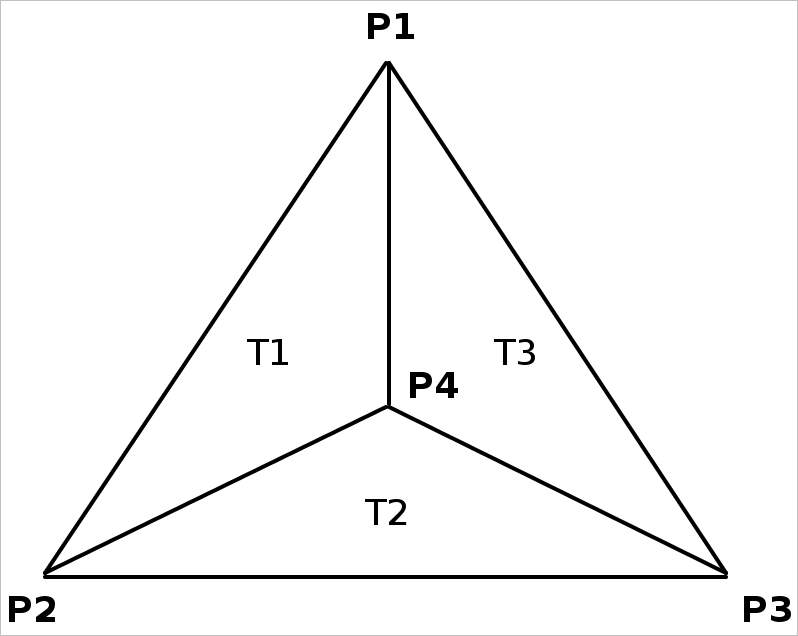
\includegraphics[width=0.7\textwidth]{./graphics/quassi-bubble}
%
\end{center}
\caption
{Transformation of triangular element T into a quasi-bubble triangle.}
\label{fig:quassi-bubble}
\end{figure}

By adopting a linear discretisation, the basis functions of the triangle QB (in
the sense of finite element) are the 4 $\Psi$ linear functions defined on the
triangle T and confirming:

$\Psi_{i}(P_{j})=\delta_{ij}$

\paragraph{Quadratic triangle}

A quadratic interpolation of the velocity field is a well-known solution to
stability problems raised by the Ladyzhenskaya-Babu\v{s}ka-Brezzi condition in
Navier--Stokes equations (also called discrete inf-sup condition). The pressure
(or the depth in Shallow Water equations) remains linear. For quadratic
interpolation, we add 3 degrees of freedom, numbered 4, 5 and 6 on Figure
quadratic.

\begin{figure}[H]%
\begin{center}
%
  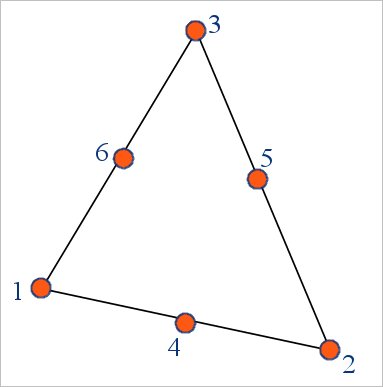
\includegraphics[width=0.7\textwidth]{./graphics/quadratic-triangle}
%
\end{center}
\caption
{quadratic triangle.}
\label{fig:quadratic-triangle}
\end{figure}

The coordinates of the 6 degrees of freedom are:
\begin{itemize}
  \item Point 1: (0,0)
  \item Point 2: (1,0)
  \item Point 3: (0,1)
  \item Point 4: (1/2,0)
  \item Point 5: (1/2,1/2)
  \item Point 6: (0,1/2)
\end{itemize}

The quadratic interpolation polynoms $P_{i} (x, y)$, with $i=1...6$, are such
that $P_{i} (x, y)=\varphi _{i} (T^{-1} (x, y))$ where $T$ is the
isoparametric transformation that gives the real triangle as a function of the
reference triangle and $\varphi _{i} $ are the basis functions in the reference
triangle. In practice $T^{-1} $ is never built and the computation of integrals
is done in the reference triangle.

The 6 quadratic basis $\varphi _{i} (\alpha , \beta )$ are chosen to ensure
the following property:
\[\mathop{\sum }\limits_{i=1}^{6} \varphi _{i} (\alpha , \beta )=1, \forall
(\alpha , \beta )\in triangle\]
Moreover every basis must be equal to 1 on its own point and zero on the five
others. This is verified if we take:
\[{\rm For\; }i=1, 2, 3{\rm ,\; }\varphi _{i} (\alpha , \beta )=(2\times
\lambda _{i} (\alpha , \beta )-1)\times \lambda _{i} (\alpha , \beta )\]
\[{\rm \; and\; for\; }i=4, 5, 6{\rm ,\; }\varphi _{i} (\alpha , \beta
)=4\times \lambda _{k} (\alpha , \beta )\times \lambda _{l} (\alpha , \beta
)\]
where \textit{k} and \textit{l} are the indices of points of the segment where
is point \textit{i}. More precisely:


\[\varphi _{1} (\alpha , \beta )=(2\times \lambda _{1} (\alpha , \beta
)-1)\times \lambda _{1} (\alpha , \beta )\]
\[\varphi _{2} (\alpha , \beta )=(2\times \lambda _{2} (\alpha , \beta
)-1)\times \lambda _{2} (\alpha , \beta )\]
\[\varphi _{3} (\alpha , \beta )=(2\times \lambda _{3} (\alpha , \beta
)-1)\times \lambda _{3} (\alpha , \beta )\]
\[\varphi _{4} (\alpha , \beta )=4\times \lambda _{1} (\alpha , \beta
)\times \lambda _{2} (\alpha , \beta )\]
\[\varphi _{5} (\alpha , \beta )=4\times \lambda _{2} (\alpha , \beta
)\times \lambda _{3} (\alpha , \beta )\]
\[\varphi _{6} (\alpha , \beta )=4\times \lambda _{3} (\alpha , \beta
)\times \lambda _{1} (\alpha , \beta )\]
\underbar{Remark:} on boundaries a point number 3 is added in the middle and
the interpolation polynoms are:
\[\begin{array}{lllll}
  {\varphi _{1} (\xi )} & {=} & {2\times (1-\xi )} & {\times } & {({\textstyle\frac{1}{2}} -\xi )} \\
  {\varphi _{2} (\xi )} & {=} & {(2\times \xi -1)} & {\times } & {\xi } \\
  {\varphi _{3} (\xi )} & {=} & {4\times \xi } & {\times } & {(1-\xi )}
\end{array}\]

\paragraph{Quadrilateral Q1}

The reference square is comprised of the coordinate points (-1,-1)  (1,-1)  (1,1) and (-1,1). On this reference element, the base functions have the following values:

$P1(\xi,\eta) = ( 1 - \xi- \eta + \xi\eta)/4$

$P2(\xi,\eta) = ( 1 + \xi- \eta - \xi\eta)/4$

$P3(\xi,\eta) = ( 1 + \xi+ \eta + \xi\eta)/4$

$P4(\xi,\eta) = ( 1 - \xi+ \eta - \xi\eta)/4$

\paragraph{Tetrahedron}

So far real there is no module in the Telemac system which fully uses this
element. In \telemac{3D} and Estel-3Dmeshes of tetrahedrons are not accepted
in.

The reference tetrahedron is comprised of the coordinate points:

(0,0,0)  (1,0,0)  (0,1,0)  (0,0,1). On this reference element, the base
functions have the following values:
\[\Psi _{1} =(1-\alpha -\beta -\gamma )\]
\[\Psi _{2} =\alpha \]
\[\Psi _{3} =\beta \]
\[\Psi _{4} =\gamma \]

\paragraph{Prism}

This is a prism with 3 vertical rectangular faces, and two triangular faces,
one at the bottom and one at the top, and which are not necessarily horizontal.

    (The figures indicate local numbering of the nodes).
\begin{figure}[H]%
\begin{center}
%
  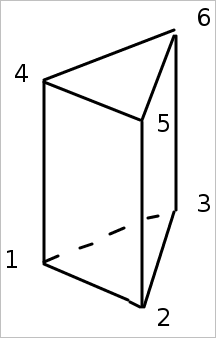
\includegraphics[width=0.7\textwidth]{./graphics/prism-numbering}
%
\end{center}
\caption{Numbering of nodes in a prism}
\label{fig:prismnumbering}
\end{figure}

The reference element is as follows:

(the figures in circles indicate local numbering of the nodes).

\begin{figure}[H]%
\begin{center}
%
  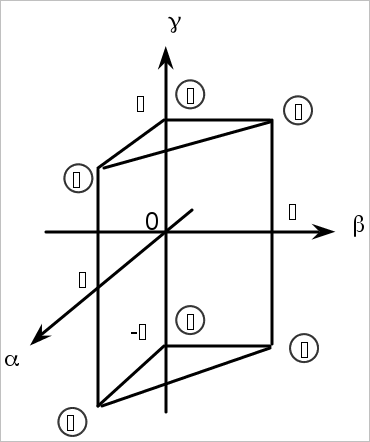
\includegraphics[width=0.7\textwidth]{./graphics/prism}
%
\end{center}
\caption{Reference element for a prism}
\label{fig:prism}
\end{figure}

The basis functions $\Psi _{j}$ corresponding to the nodes j of the reference
element are:
\[\Psi _{1} =(1-\alpha -\beta )\left(\frac{1-\gamma }{2} \right)\]
\[\Psi _{2} =\alpha \left(\frac{1-\gamma }{2} \right)\]
\[\Psi _{3} =\beta \left(\frac{1-\gamma }{2} \right)\]
\[\Psi _{4} =(1-\alpha -\beta )\left(\frac{1+\gamma }{2} \right)\]
\[\Psi _{5} =\alpha \left(\frac{1+\gamma }{2} \right)\]
\[\Psi _{6} =\beta \left(\frac{1+\gamma }{2} \right)\]

The basis functions $\phi _{i}$ on any prism in the $\omega$ mesh are obtained
by creating the $\Psi _{i}$ functions with the isoparametric transformation F,
transforming the reference prism into this prism of any type.

For a prism in the $\omega$ mesh with vertex coordinates (xi,yi,zi), F makes
any point M0 with coordinates ($\alpha$,$\beta$,$\gamma$) of the reference
element correspond to any point M with coordinates (x,y,z) of this prism by:
\[\left\{\begin{array}{c} {x=\sum _{i=1}^{6}x_{i} \Psi _{i} (\alpha ,\beta
  ,\gamma ) } \\ {y=\sum _{i=1}^{6}y_{i} \Psi _{i} (\alpha ,\beta ,\gamma ) }
  \\ {z=\sum _{i=1}^{6}z_{i} \Psi _{i} (\alpha ,\beta ,\gamma ) }
  \end{array}\right. \]
The $\Psi _{i}$ functions which appear in the definition of F are the same as
the basis functions defined on the reference element since the reference
element chosen is isoparametric (the interpolation nodes are also the geometric
nodes). In our case, the expressions of F can be simplified since:
\begin{verbatim}
 x1 = x4 ; y1 = y4
 x2 = x5 ; y2 = y5
 x3 = x6 ; y3 = y6
\end{verbatim}

The following is therefore obtained for F :
\[\left\{\begin{array}{c} {x=(1-\alpha -\beta )x_{1} +\alpha x_{2} +\beta x_{3}
  } \\ {y=(1-\alpha -\beta )y_{1} +\alpha y_{2} +\beta y_{3} } \\
  {z=\left[(1-\alpha -\beta )z_{1} +\alpha z_{2} +\beta z_{3}
  \right]\left[\frac{1-\gamma }{2} \right]+\left[(1-\alpha -\beta )z4+\alpha
  z_{5} +\beta z_{6} \right]\left[\frac{1+\gamma }{2} \right]}
  \end{array}\right. \]
  The following is deduced for the $\Phi _{i}$ functions:
  $\phi _{i} (x, y, z) =  \Psi _{i} (F-1 (x, y, z))$

\subsection{Description of mesh}

NB: The variables written in capitals are those used in the \bief FORTRAN
program. When a variable is also a component of the BIEF\_MESH structure, it is
mentioned into commas. For example on the line hereafter (MESH\%NELEM) means
that NELEM can be retrieved from a BIEF\_MESH structure by the component
NELEM..

A mesh is composed of NELEM elements (MESH\%NELEM) and NPOIN nodes
(MESH\%NPOIN) known by their coordinates X, Y, Z (respectively MESH\%X, Y and
Z). Each type of element (triangle P1,prism P0,...) is linked to a code and
includes NDP nodes. (MESH\%NDP) On an element, the nodes are numbered from 1 to
NDP. The connection between this element numbering (local numbering) and the
numbering of the mesh nodes from 1 to NPOIN (general numbering) is made through
the connectivity table IKLE (MESH\%IKLE). The global number of the node with
the local number ILOC in the element IELEM is IKLE(IELEM,ILOC).

\begin{table}[H]
\begin{center}
%
\caption{Elements in \bief version 6.2 (the \telemac{3D} prism is a prism with
four vertical quadrangular sides). Quadrilateral elements are kept for an
internal use by \telemac{3D} but no longer maintained.}
\label{tab:elemntbief}
\begin{tabular}{|p{2.4in}|p{0.8in}|} \hline
IELM & NDP(IELM) \\ \hline
00 (segment P0 = constant value) & 1 \\ \hline
01 (segment P1 = linear) & 2 \\ \hline
10 (triangle P0 = constant value) & 1 \\ \hline
11 (triangle P1 = linear) & 3 \\ \hline
12 (quasi-bubble triangle) & 4 \\ \hline
13 (quadratic element) & 6 \\ \hline
20 (quadrilateral Q0 = constant value) & 1 \\ \hline
21 (quadrilateral Q1 = linear) & 4 \\ \hline
30 (tetrahedron T0 = constant value & 1 \\ \hline
31 (tetrahedron T1 = linear & 4 \\ \hline
40 (prism P0 = constant value) & 1 \\ \hline
41 (prism P1 = linear) & 6 \\ \hline
50 (tetrahedron T0 from split prism) & 1 \\ \hline
51 (tetrahedron T1 from split prism) & 4 \\ \hline
60 (triangle P0 in a lateral boundary\newline of a mesh of prisms split into\newline tetrahedrons) & 1 \\ \hline
61 (triangle P1 in a lateral boundary\newline of a mesh of prisms split into\newline tetrahedrons) & 3 \\ \hline
70 (quadrilateral Q0 in a lateral\newline boundary of a mesh of prisms) & 1 \\ \hline
71 (quadrilateral Q1 in a lateral\newline boundary of a mesh of prisms) & 4 \\ \hline
80 (triangle P0 in a boundary\newline of a mesh of tetrahedrons) & 1 \\ \hline
81 (triangle P1 in a boundary\newline of a mesh of tetrahedrons) & 3 \\ \hline
\end{tabular}
\end{center}
\end{table}

In addition, the boundary points of the mesh must be known. These are numbered
from 1 to NPTFR (MESH\%NPTFR). The connection with the general numbering is
made through the table NBOR (MESH\%NBOR). NBOR(IPTFR) is the general number of
the boundary point IPTFR.

The tables X, Y, Z, IKLE and NBOR are sufficient for defining the mesh.
However, it is useful to have other tables available, which can often
facilitate the writing of the algorithms. Thus, is it very useful to have
tables other than NBOR to describe the boundaries. In fact, three types of
numbering can be associated with the boundary of the studied domain. These are
the boundary point numbers, the boundary face numbers and the local numbers of
the boundary nodes in each of the boundary faces. To connect them, \bief uses
IKLBOR (BIEF\%IKLBOR), a connectivity table for the boundary faces, NELBOR
(MESH\%NELBOR) linking the boundary face numbers to the element numbers to
which they belong, and NULONE (MESH\%NULONE), a table linking the local numbers
of the boundary nodes in the boundary faces to the local numbers of these nodes
in the elements to which they belong. The following example illustrates the use
of these tables for a triangular element:

\begin{figure}[H]%
\begin{center}
%
  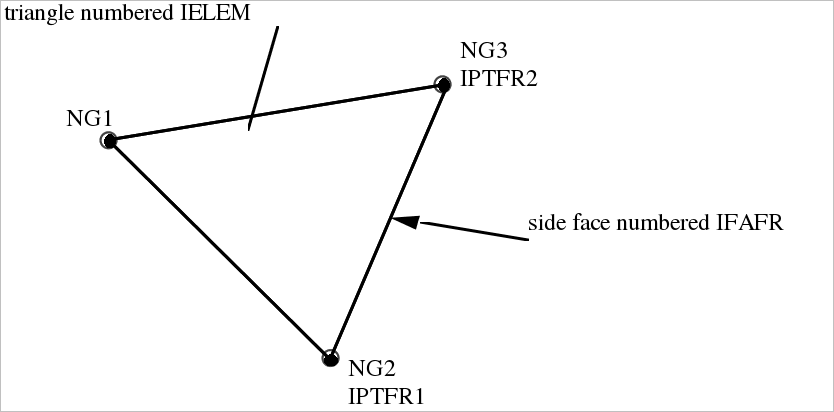
\includegraphics[width=0.7\textwidth]{./graphics/triangle}
%
\end{center}
\caption{numbering of points and faces on boundaries}
\label{fig:triangle}
\end{figure}

Take a triangle P1 numbered IELEM constructed on the 3 nodes with global
numbers NG1, NG2, NG3. The face defined by the two points NG2 and NG3 is a
boundary face with the number IFAFR. The nodes NG2 and NG3 are boundary nodes
with the boundary numbers IPTFR1 and IPTFR2. The nodes NG1, NG2 and NG3 have
the local numbers 1, 2 and 3 in the triangle. Finally, the nodes IPTFR1 and
IPTFR2 have the local numbers 1 and 2 in the boundary face.

We have:
\begin{lstlisting}[language=TelFortran]
   IKLE(IELEM,1) = NG1
   IKLE(IELEM,2) = NG2
   IKLE(IELEM,3) = NG3

   NBOR(IPTFR1) = NG2
   NBOR(IPTFR2) = NG3

   NELBOR(IFAFR) = IELEM

   IKLBOR(IFAFR,1) = IPTFR1
   IKLBOR(IFAFR,2) = IPTFR2

   NULONE(IFAFR,1) = 2
   NULONE(IFAFR,2) = 3
\end{lstlisting}

For certain elements (prisms), the boundary faces are of two types. Thus, the
boundary faces of the prism are triangles or quadrilaterals. A dimension is
then added to the tables NELBOR, IKLBOR and NULONE in order to distinguish the
type of face in question.

To know the types of boundary faces (segment P1, triangle P1...) for example to
calculate boundary matrices, a function IELBOR is used. IELBOR(IELM,1) gives
the code of the first type of face of the type IELM element (bottom and top of
prisms), IELBOR(IELM,2).gives the type of vertical sides of boundary prisms,
which may be triangles or quadrilaterals depending on the fact that the prisms
are split into tetrahedrons or not.

The adaptive mesh is simply specified by dimensioning with the maximum possible
number of NELMAX elements or the maximum possible number of NELBRX boundary
elements all the tables with several dimensions such as IKLE, NULONE...etc.

\subsection{Storage of matrices}

The theoretical aspects of "Element By Element" and ``Edge based'' storage are
discussed below. The resulting conventions are given in appendix 1.

\paragraph{EBE storage}

In a finite element code using iterative resolution methods, a matrix is
essentially used to multiply it by a vector. Other operations with a matrix are
less frequent, and, as will be seen in Chapter IV, these operations can be
constructed on the architecture of a matrix-vector product. The storage mode of
a matrix has thus been motivated in order to make its vector product as
effective as possible.

It is well known that it is not necessary to assemble a finite element matrix
to multiply it by a vector. On a mesh of NELEM elements, a matrix M is written
as a function of the elementary matrices $M_{e}$ on each of the elements according
to the following:
\[M=\prod _{e=1}^{NELEM}P_{e} M_{e} P_{e}^{t}  \]
where $P_{e}$ is a transfer matrix between the element and the general mesh.
$P_{e}$ is constructed using the connectivity table. For example, for a
triangle P1 with element number IELEM and vertices with general numbers NG1,
NG2 and NG3, MIELEM is a matrix 3*3 and PIELEM is a matrix NPOIN*3 such that
the coefficient of PIELEM situated at the intersection of row I and column J is
1 if I = IKLE(IELEM,J) and otherwise it is 0.

$P_{IELEME}=\left(
  \begin{array}{ccc}
    0 & 0 & 0 \\
    1 & 0 & 0 \\
    . & . & . \\
    0 & 1 & 0 \\
    . & . & . \\
    . & . & . \\
    . & . & . \\
    0 & 0 & 1 \\
    0 & 0 & 0
  \end{array}
\right)
  \begin{array}{c}
    \\
    line IKLE(IELEM,1) \\
    \\
    line IKLE(IELEM,2) \\
    \\
    \\
    \\
    line IKLE(IELEM,3) \\
    \\
  \end{array}
$


If X is a vector, the product M.X becomes:$MX=\prod _{e=1}^{NELEM}(P_{e} M_{e}
P_{e}^{t} )X $

which is the same as multiplying $M_{e}$ by the components of X associated with the
nodes of the element e (elementary products), then calculating the sum for all
the mesh elements (assembly). It is of course never necessary to construct the
matrix $P_{e}$ which is no other than the connectivity table IKLE.

A matrix M can be stored in the form of NELEM matrices Me. For a mesh of
triangles P1, this gives 9*NELEM coefficients. This number can be reduced by
retaining only the off-diagonal terms for each elementary matrix and assembling
the diagonal terms as shown below.

Let $D_{e}$ and $E_{e}$ the diagonal and off-diagonal parts of $M_{e}$ ($M_{e}
= D_{e} + E_{e}$), then:
\[MX=\prod _{e=1}^{NELEM}(P_{e} D_{e} P_{e}^{t} )X+\prod _{e=1}^{NELEM}(P_{e}
E_{e} P_{e}^{t} )X  =DX+\prod _{e=1}^{NELEM}(P_{e} E_{e} P_{e}^{t} )X \]

where D is the diagonal of M, obtained by assembling the diagonals De.

In \bief, a matrix MAT is therefore stored in two arrays, one being DMAT,
containing the diagonal of the assembled matrix, and the other XMAT, containing
the off-diagonal terms of the elementary matrices. For a matrix constructed on
a mesh of triangles P1, all that has to be stored is 6*NELEM + NPOIN
coefficients, which represents a saving in space of about 2.5*NELEM
coefficients compared with complete storage of the element matrices.

In addition, by using elementary matrices, it is possible to obtain a
vectorisable matrix vector product on a vector computer. The loop on the
elementary products is vectorisable and the assembly loop for these elementary
products may also be vectorisable provided a few precautions are taken
concerning the numbering of the mesh. We shall look in greater detail at the
matrix-vector product and assembly in Chapter~IV, which deals with matrix
operations.

For storage of off-diagonal elements, the convention adopted in \bief is as
follows. Let us take the case of an element IELEM constructed on NLOC nodes. An
elementary matrix Me includes in this case NLOC*(NLOC-1) off-diagonal terms
Ei,j, situated in row i and column j of Me.

Let:
\begin{lstlisting}[language=TelFortran]
XMAT(IELEM,1) = E1,2
XMAT(IELEM,2) = E1,3

.........................................

XMAT(IELEM,NLOC-1) = E1,NLOC

.........................................

XMAT(IELEM,NLOC*(NLOC-1)/2) = ENLOC-1,NLOC
\end{lstlisting}

For the terms in the upper triangular part of Me. If Me is symmetrical, the
array XMAT is complete. Otherwise, the lower triangular part of Me must also be
stored, which is achieved in the following way:
\begin{lstlisting}[language=TelFortran]

XMAT(IELEM,NLOC*(NLOC-1)/2 + 1) = E2,1

XMAT(IELEM,NLOC*(NLOC-1)/2 + 2) = E3,1

.........................................

XMAT(IELEM,NLOC*(NLOC-1)/2+ NLOC - 1) = ENLOC,1

.........................................

XMAT(IELEM,NLOC*(NLOC-1)) = ENLOC,NLOC-1
\end{lstlisting}

A matrix MIELEM constructed on a triangle P1 is thus written as a function of
XMAT as follows (the * indicate the diagonal terms which are stored elsewhere
since they are assembled):
$M_{IELEM}=
\left(
\begin{array}{ccc}
        *       & XMAT(IELEM,1) & XMAT(IELEM,2) \\
  XMAT(IELEM,4) &       *       & XMAT(IELEM,3) \\
  XMAT(IELEM,5) & XMAT(IELEM,6) &       *
\end{array}
 \right)$

The following table summarises, for a few types of elements, the memory space required for storing a matrix (for reference purposes, the space needed for compact storage is indicated).

\begin{tabular}{|p{1.3in}|p{2.2in}|p{1.2in}|} \hline
Type of element & \bief storage & Compact storage \\ \hline
Quadrilateral Q1 & NPOIN+12 NELEM=13 NPOIN & 19 NPOIN \\ \hline
Triangle P1 & NPOIN+  6 NELEM=13 NPOIN & 15 NPOIN \\ \hline
Triangle P2 & NPOIN+30 NELEM=16 NPOIN & 24 NPOIN \\ \hline
Quadrilateral Q2 (9 nodes) & NPOIN+72 NELEM=19 NPOIN & 33 NPOIN \\ \hline
Brick P1 & NPOIN+56 NELEM=57 NPOIN & 55 NPOIN \\ \hline
Prism \telemac{3D} & NPOIN+30 NELEM=61 NPOIN & 43 NPOIN \\ \hline
\end{tabular}

\paragraph{EDGE-BASED storage}

Edge-based storage is a recent technique which enables to store a matrix in an
optimal and easy way. The idea is that the element of the matrix, let's say
e.g. $\int _{\Omega }\Psi _{i}  \Psi _{j} d\Omega $, with i different from j,
is not equal to 0 only if points I and j are linked by a segment of the mesh.
Every segment is thus the best location to store these off-diagonal terms. For
a non symmetrical matrix, there will be two coefficients to store on every
segment, for a symmetrical matrix, only one will be necessary. This can be
extended to complex elements such as quasi-bubble by adding the relevant
segments. The data structure to deal with such a storage is very simple:

An array called GLOSEG, equivalent of IKLE for elements, which gives the global
numbers of the two ends of the segment. Its dimension in Fortran is (NSEG,2)
where NSEG is the total number of segments, i.e. for triangles :
(3*NELEM+NPTFR)/2.

An array called ELTSEG, with dimensions (NELEM,NS), where NS is the number of
segments in an element.(3 for a triangle). ELTSEG gives for every element the
segment numbers of its 3 segments.

An array ORISEG, with dimensions (NELEM,NS). ORISEG gives the orientation of
every segment in an element, i.e. it is equal to 1 if the segment is in
counter-clockwise orientation (from its point 1 to its point 2), and is equal
to 2 otherwise.

A matrix storage then consists of:
\begin{itemize}
  \item A diagonal
  \item Two arrays XA1 and XA2 of size NSEG.
\end{itemize}

XA1 contains the coefficient of point 2 in equation of point 1, and XA2 its
symmetrical part, coefficient of point 1 in equation of point 2.

XA2 is not necessary if the matrix is symmetrical. When the matrix is
rectangular, XA2 first contains the part symmetrical to XA1, then the extra
terms, each one corresponding with a segment and with the same order as the
segments.

The matrix thus stored is assembled.

The local numbering of segments in an element is the following:

\textbf{Linear triangle:}

Segment 1 goes from point 1 to point 2 or from point 2 to point 1 (depending of ORISEG)
Segment 2 goes from point 2 to point 3 or from point 3 to point 2 (depending of ORISEG)
Segment 3 goes from point 3 to point 1 or from point 1 to point 3 (depending of ORISEG)

\textbf{Quasi-bubble triangle:}

Segment 1 goes from point 1 to point 2 or from point 2 to point 1 (depending of ORISEG)
Segment 2 goes from point 2 to point 3 or from point 3 to point 2 (depending of ORISEG)
Segment 3 goes from point 3 to point 1 or from point 1 to point 3 (depending of ORISEG)
Segment 4 goes from point 1 to point 4
Segment 5 goes from point 2 to point 4
Segment 6 goes from point 3 to point 4

Segments 4 to 6 need no value of ORISEG, they always go from a linear point to
the quadratic point. This is used in matrix-vector products algorithms, see
subroutine MVSEG.

\textbf{Quadratic triangle:}

Segment 1 goes from point 1 to point 2 or from point 2 to point 1 (depending of ORISEG)
Segment 2 goes from point 2 to point 3 or from point 3 to point 2 (depending of ORISEG)
Segment 3 goes from point 3 to point 1 or from point 1 to point 3 (depending of ORISEG)
Segment 4 goes from point 1 to point 4
Segment 5 goes from point 2 to point 5
Segment 6 goes from point 3 to point 6
Segment 7 goes from point 2 to point 4
Segment 8 goes from point 3 to point 5
Segment 9 goes from point 1 to point 6
Segment 10 goes from point 1 to point 5
Segment 11 goes from point 2 to point 6
Segment 12 goes from point 3 to point 4
Segment 13 goes from point 4 to point 5
Segment 14 goes from point 5 to point 6
Segment 15 goes from point 6 to point 4

ORISEG is not useful for segments 4 to 15. For segments 4 to 12 the principle
is that the first point is linear (1, 2 or 3) and the second is quadratic (4, 5
or 6). Note that in rectangular linear-quadratic matrices, segments 13, 14 and
15 will not appear as they link only quadratic points. This is why they have
been put at the end, so that we have no gap in segment numbering for
rectangular matrices.

The total number of segments 4 to 6 is NSEG.

The total number of segments 7 to 9 is NSEG.

The total number of segments 10 to 11 is 3 NELEM

The total number of segments 13 to 15 is 3 NELEM

Quadratic boundary segments have also a local numbering. Point 1 and point 2
are defined as in lilnear segments, point 3 is in the middle.

\textbf{Linear prism:}

Horizontal segments:

Segment 1 goes from point 1 to point 2 or from point 2 to point 1 (depending of ORISEG)
Segment 2 goes from point 2 to point 3 or from point 3 to point 2 (depending of ORISEG)
Segment 3 goes from point 3 to point 1 or from point 1 to point 3 (depending of ORISEG)
Segment 4 goes from point 4 to point 5 or from point 5 to point 4 (depending of ORISEG)
Segment 5 goes from point 5 to point 6 or from point 6 to point 5 (depending of ORISEG)
Segment 6 goes from point 6 to point 4 or from point 4 to point 6 (depending of ORISEG)

Vertical segments:

Segment 7 goes from point 1 to point 4
Segment 8 goes from point 2 to point 5
Segment 9 goes from point 3 to point 6

Crossed segments (for their global numbering see subroutine STOSEG41):

Segment 10 goes from point 1 to point 5
Segment 11 goes from point 2 to point 4
Segment 12 goes from point 2 to point 6
Segment 13 goes from point 3 to point 5
Segment 14 goes from point 3 to point 4
Segment 15 goes from point 1 to point 6

\section{Construction of matrices}

The \bief matrices are calculated exactly through analytical integration. The
terms of a finite element matrix are generally polynomial integrals, which can
be estimated through successful completion of the analytical integration. On
paper, the analytical integration is long, tedious and a source of error, even
though it is possible to take a few short cuts. This is why we prefer the
formal calculation software programme MAPLE V, which can give in FORTRAN
the exact result of an integral calculation.

An example is given below of a matrix calculation as it can be carried out with
MAPLE V. The full description is given in the reference \citet{HervouetMaple}.

\subsection{Example of a mass-matrix calculation}

As an example, we choose here to calculate the mass matrix on a mesh of
quadrilaterals Q1. It is a little more complicated than linear triangles, but
will show that the Jacobian of isoparametric transformations is not always a
constant.

It is sufficient to conduct the calculation on a quadrangle Q with vertices P1,
P2, P3, P4 with coordinates (x1,y1), (x2,y2), (x3,y3) and (x4,y4). The element
Mi,j of the elementary mass matrix is written as follows:$M_{i,j} =\int
_{Q}\Psi _{i}  \Psi _{j} dQ$.

where $\Psi _{i}$ is the base function associated with the node i (i=1,2,3 or
4).

We thus calculate the integral on a reference element thanks to an
isoparametric transform T. Any point of the reference element Q0 with
coordinates ($\xi$,$\eta$) is associated with a point on the quadrilateral Q
with coordinates (x,y) such that:
$\left\{
  \begin{array}{l}
x(\xi,\eta) = t_{1} + t_{2}\xi + t_{3}\eta + t_{4}\xi\eta \\
y(\xi,\eta) = t'_{1} + t'_{2}\xi + t'_{3}\eta + t'_{4}\xi\eta
\end{array}\right.$

\begin{figure}[H]%
\begin{center}
%
  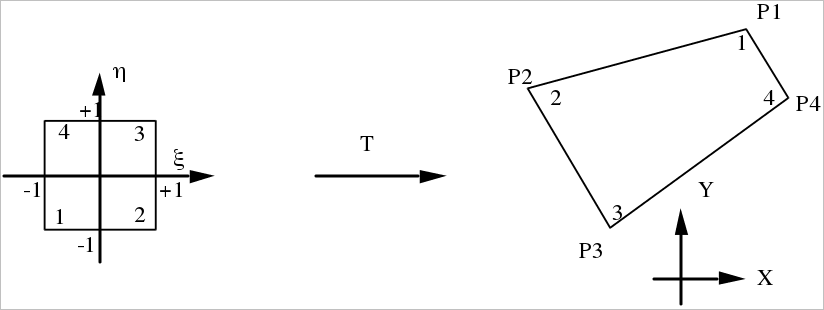
\includegraphics[width=0.7\textwidth]{./graphics/isoparametric}
%
\end{center}
\caption{Isoparametric transformation (the numbers in the quadrilaterals
indicate local numbering)}
\label{fig:isoparametric}
\end{figure}

The image by T of each vertex of the reference element thus gives a vertex of
the quadrilateral, which, by identification, provides the coefficients t1, t2,
... of the transformation, as a function of the coordinates x1,y1    x2,y2
x3,y3    x4,y4    of the vertices:

$t_{1} = ( +x1 + x2 + x3 + x4 ) / 4$

$t_{2} = ( -x1 + x2 + x3 - x4 ) / 4$

$t_{3} = ( -x1 - x2 + x3 + x4 ) / 4$

$t_{4} = ( +x1 - x2 + x3 - x4 ) / 4$

$t'_{1} = ( +y1 + y2 + y3 + y4 ) / 4$

$t'_{2} = ( -y1 + y2 + y3 - y4 ) / 4$

$t'_{3} = ( -y1 - y2 + y3 + y4 ) / 4$

$t'_{4} = ( +y1 - y2 + y3 - y4 ) / 4$

A base $\Psi$ in the real element corresponds in the reference element to a
polynomial P such that $\Psi(x,y)  =  T(P(\xi,\eta)$).

In our case, there are 4 polynomials associated with the 4 bases of the real element:

$P1(\xi,\eta) = ( 1 - \xi- \eta + \xi\eta)/4$

$P2(\xi,\eta) = ( 1 + \xi- \eta - \xi\eta)/4$

$P3(\xi,\eta) = ( 1 + \xi+ \eta + \xi\eta)/4$

$P4(\xi,\eta) = ( 1 - \xi+ \eta - \xi\eta)/4$

As for the bases $\Phi$, each polynomial has a value of 1 for one vertex of the
element and 0 for the others.

In the reference element, the integral being sought takes the value:

\[\int _{Q}\Psi _{i}  \Psi _{j} dQ=\int _{-1}^{+1}\int _{-1}^{+1}P_{i} P_{j} \left|J\right|d\xi d\eta   \]
where J is the Jacobian of the transformation T , equal to the determinant of the Jacobian matrix:

\[
\begin{array}{cc}
  \frac{\partial{x}}{\partial{\xi}} & \frac{\partial{x}}{\partial{\eta}} \\
  \\
  \frac{\partial{y}}{\partial{\xi}} & \frac{\partial{y}}{\partial{\eta}}
\end{array}
\]

Let:

$J = (t_{2}+t_{4}\eta) (t'_{3}+t'_{4}\xi) - (t'_{2}+t'_{4}\eta) (t_{2}+t_{4}\xi)$

J is assumed to be positive, which is obtained with local numbering of the
points which run along the boundary of the element in the counter-clockwise
sense. J is not constant (it is with linear triangles).

Since J is a polynomial, then we have the integral of a polynomial (of which
the term with the highest degree is in $\xi _{3}\eta _{3}$).

This information is sufficient for MAPLE V to successfully carry out the
calculation. For example, for this calculation of a mass matrix, the following
can be obtained:
\begin{lstlisting}[language=TelFortran]
!FORMAL CALCULATION OF A Q1 MASS MATRIX :

      MAT(1,1)=(X2*(2.*Y4+Y3)+X3*(Y4-Y2)+X4*(-Y3-2.*Y2))/36.
      MAT(1,2)=(X2*(Y4+2.*Y3)+X3*(Y4-2.*Y2)-X4*(Y3+Y2))/72.
      MAT(1,3)=(X2*Y3+X3*(Y4-Y2)-X4*Y3)/72.
      MAT(1,4)=(X2*(Y4+Y3)+X3*(2.*Y4-Y2)+X4*(-2.*Y3-Y2))/72.
      MAT(2,1)=(X2*(Y4+2.*Y3)+X3*(Y4-2.*Y2)-X4*(Y3+Y2))/72.
      MAT(2,2)=(3.*X2*Y3+X3*(Y4-3.*Y2)-X4*Y3)/36.
      MAT(2,3)=(X2*(-Y4+3.*Y3)+X3*(2.*Y4-3.*Y2)+X4*(-2.*Y3+Y2))/72.
      MAT(2,4)=(X2*Y3+X3*(Y4-Y2)-X4*Y3)/72.
      MAT(3,1)=(X2*Y3+X3*(Y4-Y2)-X4*Y3)/72.
      MAT(3,2)=(X2*(-Y4+3.*Y3)+X3*(2.*Y4-3.*Y2)+X4*(-2.*Y3+Y2))/72.
      MAT(3,3)=(X2*(-2.*Y4+3.*Y3)+3.*X3*(Y4-Y2)+X4*(-3.*Y3+2.*Y2 ))/36.
      MAT(3,4)=(X2*(-Y4+2.*Y3)+X3*(3.*Y4-2.*Y2)+X4*(-3.*Y3+Y2))/72.
      MAT(4,1)=(X2*(Y4+Y3)+X3*(2.*Y4-Y2)+X4*(-2.*Y3-Y2))/72.
      MAT(4,2)=(X2*Y3+X3*(Y4-Y2)-X4*Y3)/72.
      MAT(4,3)=(X2*(-Y4+2.*Y3)+X3*(3.*Y4-2.*Y2)+X4*(-3.*Y3+Y2))/ 72.
      MAT(4,4)=(X2*Y3+X3*(3.*Y4-Y2)-3.*X4*Y3)/36.
\end{lstlisting}
On a vector computer, the previous FORTRAN expressions, integrated in a loop on
the elements, are vectorised.

The above demonstration can also be conducted in the same way with any matrix
which gives the integral of a polynomial expression. This is the case of mass
matrices, divergence type matrices. For diffusion matrices, it is the case with
linear triangles, not with quadrilaterals.

\subsection{Matrices with a quasi-bubble element}

The matrices to be calculated are of the type:


\[M(i,j)=\int _{\Omega }f(\Psi _{j} ,\varphi _{i} ,F,G,H,U,V,W)d\Omega  \]

In these matrices, the test functions $\varphi$ and the basis functions $\Psi$
could be of two different types (P1 or Quasi-Bubble), as well as the
discretisation functions of the variables F,U,V...

Three cases are possible:

\underbar{a -  $\varphi$ and $\Psi$ are of type P1:}

This is the standard case. The elementary matrices are then composed of 9 terms
and their calculation is carried out by integration on a reference element by
using a transformation called isoparametric transformation.

\underbar{b -  $\varphi$ and $\Psi$ are Quasi-Bubble type:}

Elementary matrices of this type have 16 terms. These terms are calculated
easily on the basis of the calculation of the terms P1 thanks to the dividing
up of the triangle T into three sub-triangles. In fact, what we have is:

\[
\begin{array}{ccccccc}
M(i,j) & = & \int _{T1}f(\Psi _{j}^{T1} ,\varphi _{i}^{T1} ,F,...)d\Omega & + & \int _{T2}f(\Psi _{j}^{T2} ,\varphi _{i}^{T2} ,F,...)d\Omega & + & \int _{T3}f(\Psi _{j}^{T3} ,\varphi _{i}^{T3} ,F,...)d\Omega \\
       &   &   \mathrm{I1}                                                         &   &    \mathrm{I2}                                                        &   &   \mathrm{I3}
\end{array}
\]

where the power indices denote the restrictions of the functions on the
triangles in question.

The restrictions of the basis function of the Quasi-Bubble element to the
sub-triangles are the basis functions P1 on these sub-triangles. Calculation of
each of the integrals I1, I2, and I3 is thus obtained independently by the
method described in a. The sum of these integrals must then be determined. In
addition, the intersection of the supports of the Quasi-Bubble basis functions
is only made rarely on the three sub-triangles and often on a single
sub-triangle (off-diagonal terms). This results in the deletion of one or two
of the integrals I1, I2, and I3.

\begin{figure}[H]%
\begin{center}
%
  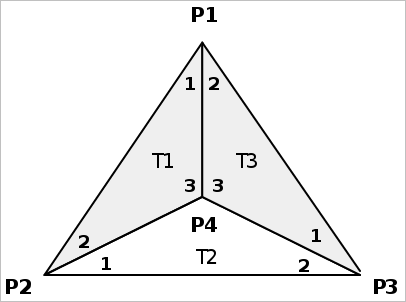
\includegraphics[width=0.7\textwidth]{./graphics/quasi-bubble-support}
%
\end{center}
\caption{Support of quasi-bubble function $\Psi _{1}$ (shaded) and local
numbering within the sub-triangles.}
\label{fig:quasibubblesupport}
\end{figure}

It can thus be observed that only the function $\Psi _{4}$ has a support which
coincides with the triangle T.

\underbar{e.g.}: calculation of the term M${}_{1,1}$:

we have:

\[
\begin{array}{ccccccc}
M_{1,1} & = & \int _{T1}f(\Psi _{1}^{T1} ,\varphi _{1}^{T1} ,F,...)d\Omega & + & 0 & + & \int _{T3}f(\Psi _{1}^{T3} ,\varphi _{1}^{T3} ,F,...)d\Omega \\
& = &            m1_{1,1}                                                  & + & 0 & + & m3_{2,2}
\end{array}
\]

m1, m2, or m3 designating the matrix P1 calculated on the sub-triangle Pi. In
fact,  is the base function assigned to the first point of the sub-triangle T1,
and  is the basis function assigned to the second point of the sub-triangle T3.

The matrix M Quasi-Bubble x Quasi-Bubble is thus finally obtained thanks to
pre-assembling of sub-matrices P1. All these operations are summarised in the
following table:
$M_{1,1} = m1_{1,1} + m3_{2,2}$

$M_{1,2} = m1_{1,2}$

$M_{1,3} = m3_{2,1}$

$M_{1,4} = m1_{1,3} + m3_{2,3}$

$M_{2,1} = m1_{2,1}$

$M_{2,2} = m1_{2,2} + m2_{1,1}$

$M_{2,3} = m2_{1,2}$

$M_{2,4} = m1_{2,3} + m2_{1,3}$

$M_{3,1} = m3_{1,2}$

$M_{3,2} = m2_{2,1}$

$M_{3,3} = m2_{2,2} + m3_{1,1}$

$M_{3,4} = m2_{2,3} + m3_{1,3}$

$M_{4,1} = m1_{3,1} + m3_{3,2}$

$M_{4,2} = m1_{3,2} + m2_{3,1}$

$M_{4,3} = m2_{3,2} + m3_{3,1}$

$M_{4,4} = m1_{3,3} + m2_{3,3} + m3_{3,3}$

\underbar{c -  $\varphi$ and $\Psi$ are of different types:}

The elementary matrices of this type are rectangular and include 12 terms.
Here, we shall deal with the case where $\varphi$ is P1 and $\Psi$
Quasi-Bubble; the symmetrical situation results directly from this.

The following can still be written:

\[
\begin{array}{ccccccc}
M(i,j) & = &\int _{T1}f(\Psi _{j}^{T1} ,\varphi _{i}^{T1} ,F,...)d\Omega & + & \int _{T2}f(\Psi _{j}^{T2} ,\varphi _{i}^{T2} ,F,...)d\Omega & + & \int _{T3}f(\Psi _{j}^{T3} ,\varphi _{i}^{T3} ,F,...)d\Omega  \\
       &   &   I1                                                         &   &    I2                                                        &   &   I3
\end{array}
\]

Unlike the situation encountered in b), the restrictions of the functions ? to
the sub-triangles no longer correspond to the base functions P1 on these
sub-triangles. In fact, what we have is:

$\varphi_{i}(P_{j})=\sigma _{ij} for 1 \le j \le 3$

and:

$\varphi_{i}(P_{4})=\frac{1}{3}$

since P${}_{4}$ is the centre of gravity of the triangle T.

In the internal numbering of the sub-triangles Ti , P${}_{4}$ always
corresponds to the point n${}^\circ$3, so that we have the following basis
functions in the reference triangle:


\begin{figure}[H]%
\begin{center}
%
  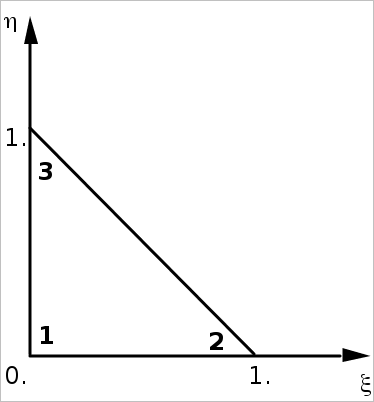
\includegraphics[width=0.7\textwidth]{./graphics/ref-triangle}
%
\end{center}
\caption{Reference element for a triangle}
\label{fig:reftriangle}
\end{figure}

\begin{tabular}{lccc}
function P & P(1) & P(2) &  P(3) \\
  $P_{1}(\xi,\eta) = 1 - \xi - \frac{2}{3} \eta$ & 1 & 0 & $\frac{1}{3}$ \\
  $P_{2}(\xi,\eta) = \xi + \frac{1}{3} \eta$ & 1 & 0 & $\frac{1}{3}$ \\
  $P_{3}(\xi,\eta) = \frac{1}{3} \eta$ & 1 & 0 & $\frac{1}{3}$
\end{tabular}

The isoparametric transformation retains the value of the functions at the
nodes, so that the anticipated result is obtained in the real mesh.

The matrix coefficients on the triangle T are obtained by assembling on the
sub-triangles:
$M_{1,1} = m1_{1,1} + m3_{2,2}$

$M_{1,2} = m1_{1,2} + m2_{3,1}$

$M_{1,3} = m2_{3,2} + m3_{2,1}$

$M_{1,4} = m1_{1,3} + m2_{3,3} + m3_{2,3}$

$M_{2,1} = m1_{1,2} + m3_{3,2}$

$M_{2,2} = m1_{2,2} + m2_{1,1}$

$M_{2,3} = m2_{1,2} + m3_{3,1}$

$M_{2,4} = m1_{2,3} + m2_{1,3} + m3_{3,3}$

$M_{3,1} = m1_{3,1} + m3_{1,2}$

$M_{3,2} = m1_{3,2} + m2_{2,1}$

$M_{3,3} = m2_{2,2} + m3_{1,1}$

$M_{3,4} = m1_{3,3} + m2_{2,3} + m3_{1,3}$

In the opposite case of a Quasi-Bubble*P1 matrix, the following would be obtained:

$M_{1,1} = m1_{1,1} + m3_{2,2}$

$M_{1,2} = m1_{1,2} + m3_{2,3}$

$M_{1,3} = m1_{1,3} + m3_{2,1}$

$M_{2,1} = m1_{2,1} + m2_{1,3}$

$M_{2,2} = m1_{2,2} + m2_{1,1}$

$M_{2,3} = m1_{2,3} + m2_{1,2}$

$M_{3,1} = m2_{2,3} + m3_{1,2}$

$M_{3,2} = m2_{2,1} + m3_{1,3}$

$M_{3,3} = m2_{2,2} + m3_{1,2}$

$M_{4,1} = m1_{3,1} + m2_{3,3} + m3_{3,2}$

$M_{4,2} = m1_{3,2} + m2_{3,1} + m3_{3,3}$

$M_{4,3} = m1_{3,3} + m2_{3,2} + m3_{3,1}$

\section{Matrix operations:}

It was shown above that matrix operations in \bief are carried out at elementary
level first of all and then assembled.

This section gives a detailed description of the assembly algorithm and the
main matrix operations carried out in \bief, in the case of an element by
element storage, namely:
\begin{itemize}
  \item Product of a non symmetrical matrix and a vector
  \item Product of a symmetrical matrix and a vector
  \item Product of the transpose of a matrix and a vector
  \item Processing of Dirichlet-type boundary conditions in the matrices
  \item Diagonal preconditioning
\end{itemize}

The main algorithm is in fact the product of a matrix and a vector, as it will
be seen that all the others can be reduced to this, or at least be derived from
it.

Then in the last section we shall detail the matrix-vector product when using
an edge-based storage.

\subsection{Assembly of an elementary vector}

With a known vector We of dimension NLOC for each element, a general vector R
of dimension NPOIN must be defined. Using the notation of chapter I, this is
written as follows:
\[R=\sum _{e=1}^{NELEM}(P_{e} W_{e} ) \]

Taking the example of the triangle P1, if the components of the vector WIELEM
are designated W1, W2, and W3 , then W1(IELEM) is the vector component at the
node with local number 1 of element IELEM, etc.

In FORTRAN, R is defined as follows:

\begin{lstlisting}[language=TelFortran]
DO IELEM=1,NELEM
  R(IKLE(IELEM,1)) = R(IKLE(IELEM,1))  +  W1(IELEM)
  R(IKLE(IELEM,2)) = R(IKLE(IELEM,2))  +  W2(IELEM)
  R(IKLE(IELEM,3)) = R(IKLE(IELEM,3))  +  W3(IELEM)
ENDDO
\end{lstlisting}

where IKLE is the connectivity table: IKLE(IELEM,I) is the general number of
the Ith local node of element IELEM.

This loop can be vectorised, as will be seen below.

The assembly loop is first of all transformed into three successive loops:

\begin{lstlisting}[language=TelFortran]
!
DO IELEM=1,NELEM
  R(IKLE(IELEM,1))=R(IKLE(IELEM,1))+W1(IELEM)
ENDDO
!
DO IELEM=1,NELEM
  R(IKLE(IELEM,2))=R(IKLE(IELEM,2))+W2(IELEM)
ENDDO
!
DO IELEM=1,NELEM
  R(IKLE(IELEM,3))=R(IKLE(IELEM,3))+W3(IELEM)
ENDDO
\end{lstlisting}

These three loops are not automatically vectorised on a vector computer.
Indeed, the principle of vectorisation is to work in real time on a number of
elements of the loop. This number, referred to as the vector length of the
computer, varies from one supercomputer to another. It is 64 or 128 on a Cray
YMP and up to 1024 on a Fujitsu. Taking the Cray as an example, a loop running
from 1 to NELEM will be processed in 64-element clusters. Thus, if loop 1 is
vectorised on a Cray computer, the instruction R(IKLE(IELEM,1))=
R(IKLE(IELEM,1)) +W1(IELEM) will be executed simultaneously for elements 1 to
64, 65 to 128 and so on. It is clear, therefore, that the result can only be
correct if each component of vector R is used only once in each cluster of 64
elements, i.e. if there are not two elements IELEM1 and IELEM2 in the same
cluster such that IKLE(IELEM1,1)=IKLE(IELEM2,1). During compilation, the Cray
will detect any problem of backward dependency and not vectorise the loop.

It is, however, possible to force vectorisation, but in this case it is
essential to ensure that the grid does not contain any backward dependencies.
This again shows the advantages of having split the initial assembly loop into
three, as otherwise the condition of non-dependency would have been more severe
and hence more difficult to achieve. It would have been necessary for
IKLE(IELEM1,I) -- IKLE(IELEM2,J) for I,J = 1,2,3 for all different elements
IELEM1, IELEM2 contained in each 64-element batch.

With a split assembly loop on the Cray, backward dependencies occurs if 2
different elements IELEM1 and IELEM2 are such that:

\begin{lstlisting}[language=TelFortran]
IELEM1/64 = IELEM2/64  !(/ here indicates the complete division)
\end{lstlisting}

and if I=1,2, or 3 such that

\begin{lstlisting}[language=TelFortran]
IKLE(IELEM1,I) = IKLE(IELEM2,I)
\end{lstlisting}

On a Fujitsu computer or similar, 64 must be replaced by 1024. The set
conditions for the grid are thus more severe.

In order to vectorise the three loops, it is necessary to find a system for
numbering the elements that eliminates any backward dependencies. This leads to
a paradoxical situation as such a numbering system is impossible in theory yet
easy to apply in practice. Indeed:
\begin{itemize}
  \item there are counter-examples if the number of elements is too small,
  \item heuristic algorithms easily find a large number of acceptable numbering
    systems if the number of elements is sufficient (in practice sufficiently
    larger than the vector length, i.e. 64 for a Cray).
\end{itemize}

A counter-example and then a "heuristic" algorithm will therefore be discussed
below.

\underbar{Counter-example:}

It is sufficient to consider a grid of triangles containing less than 64
elements, in which one point belongs to four different triangles. This point
must have the same local number (1, 2 or 3) in at least two of these triangles,
which will create a backward dependencies that is impossible to eliminate.

\underbar{Element numbering algorithm}

The basic idea is to search for dependency situations and progressively
eliminate them. Starting with an existing system (for more than 64 elements),
the algorithm goes through the numbering and examines all sequences of 64
elements. When a faulty element appears, its number is exchanged with that of a
higher-ranking element.

The algorithm fails if there are still dependencies and no higher ranking
element. In this case the numbers are exchanged with those of a lower-ranking
element, which means that the previous checks are invalidated. The entire
algorithm is therefore rerun!

In practice, this algorithm is extremely efficient and rarely has to be run
more than twice. This is due to the fact that, as soon as there are more than
several hundred elements, the combinational provides a large number of suitable
numbering systems.

Once the elements have been numbered, it is simply a question of informing the
compiler that there are no backward dependencies in the loops that it will
encounter (command CDIR\$ IVDEP on a Cray, *VOCL LOOP,NVREC on
Siemens-Fujitsu).

In the case of a large vector length, there is no guarantee that a solution
will exist for average grids (containing a few thousand elements). In order to
benefit from vectorisation, however, it is still possible to split the assembly
loops into sub-loops involving only batches of elements that contain no
backward dependencies. In this case, vectorisation is forced for all these
sub-loops.

Assuming that the following loop is valid for a vector length of 64:

\begin{lstlisting}[language=TelFortran]
!
        DO IELEM=1,NELEM
            R(IKLE(IELEM,1))=R(IKLE(IELEM,1))+W1(IELEM)
        ENDDO
!
\end{lstlisting}

it can be transposed for higher vector-lengths as follows:
\begin{lstlisting}[language=TelFortran]
!
       M64 = NELEM/64
       N64 = MOD(NELEM,64)
!
       DO K =1,M64
         DO IELEM=(K-1)*64+1,K*64
           R(IKLE(IELEM,1))=R(IKLE(IELEM,1))+W1(IELEM)
         ENDDO
       ENDDO
!
       DO IELEM=M64*64+1,M64*64+N64
         R(IKLE(IELEM,1))=R(IKLE(IELEM,1))+W1(IELEM)
       ENDDO
!
\end{lstlisting}

Vectorisation of loops 2 and 3 may be forced.

Tests on a Cray YMP show that vectorisation provides very considerable savings
in the amount of time required for vector assembly:
\begin{itemize}
  \item factor of 19 for quadrilaterals with bilinear interpolation (4 loops),
  \item factor of 12 for triangles with linear interpolation (3 loops).
\end{itemize}

As vector assembly operations are used intensively in the algorithms, the
overall amount of time saved is also appreciable (up to a factor of 3).

\subsection{Product non symmetrical matrix by vector}

The problem involves calculating the vector R, which is the product of the
matrix M and the vector V. It will be recalled that:
\[R=MV=DV+\sum _{e=1}^{NELEM}(P_{e} E_{e} P_{e}^{t} ) .V\]

The example of quadrilaterals Q1 is discussed below. The matrix M is stored in
the form of two arrays DM(NPOIN) and XM(NELEM,12).

The FORTRAN instructions are as follows:

Contribution of the diagonal: product of D and V (loop that can be expressed in vector form):

\begin{lstlisting}[language=TelFortran]
DO I=1,NPOIN
  R(I) = DM(I) * V(I)
ENDDO
\end{lstlisting}

Contribution of off-diagonal terms: products $E_{e} (P_{e}^{t} V)$ stored in working arrays W1, W2, W3 and W4. This loop can also be expressed in vector form.

\begin{lstlisting}[language=TelFortran]
DO IELEM=1,NELEM
\end{lstlisting}

General numbers of points for the element (given by the array IKLE)

\begin{lstlisting}[language=TelFortran]
  I1 = IKLE(IELEM,1)
  I2 = IKLE(IELEM,2)
  I3 = IKLE(IELEM,3)
  I4 = IKLE(IELEM,4)
\end{lstlisting}

As far as the element is concerned, the results concerning points with different local numbers are stored separately (for numbers 1: W1,  etc.)

\begin{lstlisting}[language=TelFortran]
  W1(IELEM) = + XM(IELEM, 1) * V(I2)
              + XM(IELEM, 2) * V(I3)
              + XM(IELEM, 3) * V(I4)

  W2(IELEM) = + XM(IELEM, 7) * V(I1)
              + XM(IELEM, 4) * V(I3)
              + XM(IELEM, 5) * V(I4)

  W3(IELEM) = + XM(IELEM, 8) * V(I1)
              + XM(IELEM,10) * V(I2)
              + XM(IELEM, 6) * V(I4)

  W4(IELEM) = + XM(IELEM, 9) * V(I1)
              + XM(IELEM,11) * V(I2)
              + XM(IELEM,12) * V(I3)

ENDDO
\end{lstlisting}

The vector defined by W1, W2, W3 and W4 is assembled and then added to R, which
already contains the contribution of the diagonal.

This algorithm is very easy to explain. Taking as an example the term
XM(IELEM,1), this is conventionally the term MAT(1,2) for element IELEM. It is
thus a part of the coefficient of point 2 of element IELEM in the equation for
point 1 of the same element. The product XM(IELEM,1)*V(I2) must therefore be
added to the result R(I1). This is what happens in loop 2 and the assembly loop
via working array W1.

To summarise the method, it may be said that the vectors, and no longer the
matrices, are assembled. In a method involving classical compacting,
vectorisation of the product matrix x vector is broken by an internal loop on
the surrounding points.

\subsection{Product symmetrical matrix by vector}

When the matrix is symmetrical, the terms XM(IELEM,NLOC*(NLOC-1)/2+1) to
XM(IELEM,NLOC*(NLOC-1)) are no longer stored as they are equal respectively to
XM(IELEM,1),...,XM(IELEM,NLOC*(NLOC-1)/2).

In calculating the working arrays W1,... , they simply need to be substituted,
so that the following are obtained, still for quadrilaterals Q1:
\begin{lstlisting}[language=TelFortran]
  W1(IELEM) = + XM(IELEM,1) * V(I2)
              + XM(IELEM,2) * V(I3)
              + XM(IELEM,3) * V(I4)

  W2(IELEM) = + XM(IELEM,1) * V(I1)
              + XM(IELEM,4) * V(I3)
              + XM(IELEM,5) * V(I4)

  W3(IELEM) = + XM(IELEM,2) * V(I1)
              + XM(IELEM,4) * V(I2)
              + XM(IELEM,6) * V(I4)

  W4(IELEM) = + XM(IELEM,3) * V(I1)
              + XM(IELEM,5) * V(I2)
              + XM(IELEM,6) * V(I3)
\end{lstlisting}

\subsection{Product transposed matrix by vector}

The elementary products XM(IELEM,I) simply have to be replaced by
XM(IELEM,I+NLOC*(NLOC-1)/2) if I~$\mathrm{\le}$~NLOC*(NLOC-1)/2 and by
XM(IELEM,I-NLOC*(NLOC-1)/2) if I~$>$~NLOC*(NLOC-1)/2. This gives the following
for matrices constructed on the quadrilaterals Q1:

\begin{lstlisting}[language=TelFortran]
  W1(IELEM) = + XM(IELEM, 7) * V(I2)
              + XM(IELEM, 8) * V(I3)
              + XM(IELEM, 9) * V(I4)

  W2(IELEM) = + XM(IELEM, 1) * V(I1)
              + XM(IELEM,10) * V(I3)
              + XM(IELEM,11) * V(I4)

  W3(IELEM) = + XM(IELEM, 2) * V(I1)
              + XM(IELEM, 4) * V(I2)
              + XM(IELEM,12) * V(I4)

  W4(IELEM) = + XM(IELEM, 3) * V(I1)
              + XM(IELEM, 5) * V(I2)
              + XM(IELEM, 6) * V(I3)
\end{lstlisting}

It can be seen from the last two examples above that problems of symmetry and
transposition are simply questions of how information is written for
non-assembled storage.

\subsection{Dirichlet-type boundary conditions}
\label{ref:dirichletbnd}

The following discussion concentrates on the case in which Dirichlet-type
points are not eliminated from the equations. This is the only case that poses
any problem, as it calls for local correction of the matrix. Instead of
eliminating points that are not degrees of freedom, they are retained and
assigned an equation of the type x=prescribed value. In the other equations, 0
is taken as coefficient in places where there is a Dirichlet node, while the
right hand sides of the equations are of course also changed. In this way the
symmetry of the matrix is not modified.

In other words, for a Dirichlet-type point, 1 is placed on the matrix diagonal
and off-diagonal terms are cancelled. Starting from a point, however, there is
no data structure for quickly finding elements to which a single point belongs.
It is thus apparently impossible to cancel the related off-diagonal terms if
these have been stored by element. In spite of this, they may be cancelled with
the loop described below, which again uses the principle of the product matrix
x vector.

In the following, the vector V has a value of 1 for a normal point and 0 for a
Dirichlet point. Thus any element of the matrix that would "touch" a Dirichlet
point in a matrix x vector product is cancelled and the other elements remain
unchanged, which is the desired effect. For a matrix constructed on
quadrilaterals Q1, this gives:

\begin{lstlisting}[language=TelFortran]
DO IELEM=1,NELEM
  I1 = IKLE(IELEM,1)
  I2 = IKLE(IELEM,2)
  I3 = IKLE(IELEM,3)
  I4 = IKLE(IELEM,4)
!
  XM(IELEM, 1) = XM(IELEM, 1) * V(I2) * V(I1)
  XM(IELEM, 2) = XM(IELEM, 2) * V(I3) * V(I1)
  XM(IELEM, 3) = XM(IELEM, 3) * V(I4) * V(I1)
  XM(IELEM, 7) = XM(IELEM, 7) * V(I1) * V(I2)
  XM(IELEM, 4) = XM(IELEM, 4) * V(I3) * V(I2)
  XM(IELEM, 5) = XM(IELEM, 5) * V(I4) * V(I2)
  XM(IELEM, 8) = XM(IELEM, 8) * V(I1) * V(I3)
  XM(IELEM,10) = XM(IELEM,10) * V(I2) * V(I3)
  XM(IELEM, 6) = XM(IELEM, 6) * V(I4) * V(I3)
  XM(IELEM, 9) = XM(IELEM, 9) * V(I1) * V(I4)
  XM(IELEM,11) = XM(IELEM,11) * V(I2) * V(I4)
  XM(IELEM,12) = XM(IELEM,12) * V(I3) * V(I4)
ENDDO
\end{lstlisting}

In a non-assembled matrix, the row and column for each Dirichlet-type point are
thus cancelled, with the exception of the diagonal terms.

As there is a special array for the matrix diagonal, it is then easy to replace
an element on this diagonal by 1 whenever the point in question is of Dirichlet
type. Similarly, the set values must then be placed in the second members of
the linear system.

\subsection{Products between diagonal matrix and matrix}

These products appear in particular during diagonal or block-diagonal
preconditioning of a linear system, in which the system matrix M is replaced by
DMD, in which D is a diagonal matrix.

It is therefore necessary to obtain the products DM and MD.

In the following FORTRAN examples, D is declared to be a real array of
dimension NPOIN and D(I) represents the I${}^{th}$ element of the diagonal
matrix. As it is obvious how the diagonal of the results matrix is calculated,
only the algorithms for the off-diagonal terms will be discussed (case of
quadrilaterals Q1):

\underbar{Product DM:}

\begin{lstlisting}[language=TelFortran]
!
DO 1 IELEM = 1 , NELEM
!
  I1 = IKLE(IELEM,1)
  I2 = IKLE(IELEM,2)
  I3 = IKLE(IELEM,3)
  I4 = IKLE(IELEM,4)
!
  XM(IELEM, 1) = XM(IELEM, 1) * D(I1)
  XM(IELEM, 2) = XM(IELEM, 2) * D(I1)
  XM(IELEM, 3) = XM(IELEM, 3) * D(I1)
!
  XM(IELEM, 4) = XM(IELEM, 4) * D(I2)
  XM(IELEM, 5) = XM(IELEM, 5) * D(I2)
  XM(IELEM, 6) = XM(IELEM, 6) * D(I3)
!
  XM(IELEM, 7) = XM(IELEM, 7) * D(I2)
  XM(IELEM, 8) = XM(IELEM, 8) * D(I3)
  XM(IELEM, 9) = XM(IELEM, 9) * D(I4)
!
  XM(IELEM,10) = XM(IELEM,10) * D(I3)
  XM(IELEM,11) = XM(IELEM,11) * D(I4)
  XM(IELEM,12) = XM(IELEM,12) * D(I4)
!
ENDDO
!
\end{lstlisting}

The formula for the assembled matrices would be DM(m,n) = D(m) x M(m,n). With
XM(IELEM,1) representing for example part of the term M(I1,I2), it is therefore
logically multiplied by D(I1). For the product MD, it will be multiplied by
D(I2):

\underbar{Product MD:}

\begin{lstlisting}[language=TelFortran]
DO IELEM = 1 , NELEM
!
  I1 = IKLE(IELEM,1)
  I2 = IKLE(IELEM,2)
  I3 = IKLE(IELEM,3)
  I4 = IKLE(IELEM,4)
!
  XM(IELEM, 1) = XM(IELEM, 1) * D(I2)
  XM(IELEM, 2) = XM(IELEM, 2) * D(I3)
  XM(IELEM, 3) = XM(IELEM, 3) * D(I4)
!
  XM(IELEM, 4) = XM(IELEM, 4) * D(I3)
  XM(IELEM, 5) = XM(IELEM, 5) * D(I4)
  XM(IELEM, 6) = XM(IELEM, 6) * D(I4)
!
  XM(IELEM, 7) = XM(IELEM, 7) * D(I1)
  XM(IELEM, 8) = XM(IELEM, 8) * D(I1)
  XM(IELEM, 9) = XM(IELEM, 9) * D(I1)
!
  XM(IELEM,10) = XM(IELEM,10) * D(I2)
  XM(IELEM,11) = XM(IELEM,11) * D(I2)
  XM(IELEM,12) = XM(IELEM,12) * D(I3)
!
ENDDO
\end{lstlisting}

The result is itself in the form of a non-assembled matrix and the previous two
loops are vectorised.

\subsection{Matrix-vector product with edge-based storage}

As matrices in edge-based storage are fully assembled, the matrix-vector
product is rather easy to implement. If one wants to multiply a matrix A by a
vector Y, to get X, first the diagonal terms have to be taken into account, X
is initialised with DA Y. Then the off-diagonal terms are dealt with with the
following assembly loop:

\begin{lstlisting}[language=TelFortran]
DO ISEG=1,NSEG
  X(GLOSEG(ISEG,1))=
  X(GLOSEG(ISEG,1))+XA1(ISEG)*Y(GLOSEG(ISEG,2))
!
  X(GLOSEG(ISEG,2))=
  X(GLOSEG(ISEG,2))+XA2(ISEG)*Y(GLOSEG(ISEG,1))
ENDDO
\end{lstlisting}

For rectangular matrices, all the values of X are not initialised by the
diagonal terms, so some terms in X have to be previously set to 0.

\section{Solvers and preconditioning operations}

\bief offers several iterative methods for solving a linear system M.X=B. This
can be done with preconditioning. A single solving subroutine SOLVE (see
section A.IV) processes both cases in which M is a matrix and those in which it
is a block consisting of 4 or 9 matrices. In the subroutine SOLVE,
preconditioning and method are specified by the arguments PRECON and METHOD.

The integer PRECON may have the following values at present:

\begin{description}
  \item [0 or 1] no preconditioning

  \item [2] preconditioning with the matrix diagonal
  \item [3] block-diagonal preconditioning
  \item [5] diagonal preconditioning with absolute value of matrix diagonal
  \item [7] Crout preconditioning
  \item [11]: Gauss-Seidel EBE preconditioning
  \item [13]: Preconditioning matrix given by the user
  \item [17]: 3-diagonal solution on points on a vertical in 3D (specific to
    \telemac{3D})
\end{description}

or a combination of these values. As the basic preconditioning operations are
designated by a prime number, it can be split into PRECON prime factors in
order to determine the various preconditioning operations required by the user.
For example, PRECON=14 corresponds to combined diagonal preconditioning and
Crout preconditioning.

METHOD in an array of two integers.

The integer METHOD(1) may have the following values at present:
\begin{description}
  \item [1] for the conjugate gradient method
  \item [2] for the conjugate residualconjugate residual method
  \item [3] for the normal equationnormal equation conjugate gradientconjugate
    gradient method
  \item [4] for the minimum errorminimum error method
  \item [5] for the squared conjugate gradient method
  \item [6] for the stabilised squared conjugate gradient
    method
  \item [7] for the GMRES method
  \item [8] for a direct solution
\end{description}

The integer METHOD(2) designates an option or alternative of the selected
solver. At present, this is only used for the GMRES method and designates the
dimension of the Krylov sub-space.

The various solvers and preconditioning operations will now be described in
succession.

\subsection{The various solvers}

A direct solver has been added to library \bief from version 5.8 on (solver
number 8). As it may be changed in a near future (replaced by the software
called MUMPS) it will not be described here. Only iterative solvers are
referred to hereafter.

These are used to solve a linear system of the form A.X = B. It will be
recalled that the different methods are chosen by assigning a certain value to
the integer METHOD. All the  methods are iterative. Starting with an estimate
of the solution X0, they construct a series of vectors Xm that converge towards
the exact solution of the system (provided of course that A has the required
properties).

Preconditioning options 7, 11, 13 and 17 are the only directly involved in the
algorithms of the various solution methods. The other types of preconditioning
act on the matrix upline of the calculation. A diagonal preconditioning like 2
or 3 may be combined with another preconditioning like 7, 11 and 13. In this
case the choice is the product of both, e.g. 14 for a combination of diagonal
and Crout preconditioning.

Note: preconditioning 7, 11 and 13 may behave differently in parallel, and are
thus not recommended with domain decomposition

The algorithms for the various methods available in \bief are listed below.
(X,Y) designates the scalar product of the vectors X and Y and C is either the
identity (no preconditioning) or the Crout preconditioning matrix.

\paragraph{Conjugate gradient method (METHOD=1)}

Convergence is ensured if A is a positive symmetrical matrix.

\underbar{Initialisation operations:}

$r^{0}  =  A X^{0} - B$

solution of $Cg^{0}  =  r^{0}$

$d^{0} = g^{0}$

$\rho ^{0} = \frac{(r^{0},g^{0})}{(Ad^{0},d^{0})}$

$X^{1}  =  X^{0}  -  \rho ^{0} d^{0}$

\underbar{Iterations:}

$r^{m}  =  r^{m-1}  -  \rho ^{m-1} A d^{m-1}$

solution of $Cg^{m}  =  r^{m}$

$d^{m} = g^{m} + \frac{(r^{m},g^{m})}{(r^{m-1},g^{m-1})} d^{m-1}$

$\rho ^{m} = \frac{(r^{m},d^{m})}{(d^{m},Ad^{m})}$

$X^{m+1}  =  X^{m}  -  \rho ^{m} d^{m}$

\paragraph{Conjugate residual method (METHOD=2)}

Convergence is ensured if A is a positive symmetrical matrix.

\underbar{Initialisation operations:}

$r^{0}  =  A X^{0} - B$

solution of $Cg^{0}  =  r^{0}$

$d^{0}  =  g^{0}$

solution of $Cd'0  =  Ad^{0}$

$\rho ^{0} = \frac{(g^{0},Ad^{0})}{(d'^{0},Ad^{0})}$

$X^{1}  =  X^{0}  -  \rho ^{0} d^{0}$

\underbar{Iterations:}

$r^{m}  =  r^{m-1}  -  \rho ^{m-1} A d^{m-1}$

$g^{m}  =  g^{m-1}  -  \rho ^{m-1} d'^{m-1}$

$d^{m} = g^{m} - \frac{(Ag^{m},d'^{m-1})}{(Ad^{m-1},d'^{m-1})} d^{m-1}$

$Ad^{m} = Ag^{m} - \frac{(Ag^{m},d'^{m-1})}{(Ad^{m-1},d'^{m-1})} Ad^{m-1}$

solution of $Cd'^{m}  =  Ad^{m}$

$\rho ^{m} = \frac{(Ad^{m},g^{m})}{(Ad^{m},d'^{m})}$

$X^{m+1}  =  X^{m}  -  \rho ^{m} d^{m}$

\paragraph{Normal equation conjugate gradient method (METHOD=3)}

Convergence is ensured if A is a regular matrix.

\underbar{Initialisation operations:}

$r^{0}  =  A X^{0} - B$

solution of $Cg^{0}  =  r^{0}$

solution of $ ^{t}Cg'^{0} = g^{0}$

$d^{0}  =   ^{t}A g'^{0}$

solution of $Cd'^{0}  =  Ad^{0}$

$\rho ^{0} = \frac{(d^{0},d^{0})}{(d'^{0},d'^{0})}$

$X^{1} = X^{0}  -  \rho ^{0} d^{0}$

\underbar{Iterations:}

$r^{m}  =  r^{m-1}  -  \rho ^{m-1} A d^{m-1}$

$g^{m}  =  g^{m-1}  -  \rho ^{m-1} d'^{m-1}$

solution of $ ^{t}Cg'^{m} = g^{m}$

$d^{m} =  ^{t}Ag'^{m}
        + \frac{( ^{t}Ag'^{m}, ^{t}Ag''^{m})}
               {( ^{t}Ag'^{m-1}, ^{t}Ag'^{m-1})} d^{m-1}$

solution of $Cd'^{m}  =  Ad^{m}$

$\rho ^{m} = \frac{( ^{t}Ag'^{m}, ^{t}Ag'^{m})}{(d'^{m},d'^{m})}$

$X^{m+1}  =  X^{m}  -  \rho ^{m} d^{m}$

\paragraph{Minimum error method (METHOD=4)}

Convergence is ensured if A is a regular matrix.

\underbar{Initialisation operations:}

$r^{0}  =  A X^{0} - B$

solution of $Cg^{0}  =  r^{0}$

solution of $ ^{t}Cg'^{0}  =  g^{0}$

$d^{0}  =  ^{t}A g'^{0}$

$\rho ^{0} = \frac{(g^{0},g^{0})}{(d^{0},d^{0})}$

$X^{1}  =  X^{0}  -  \rho ^{0} d^{0}$

\underbar{Iterations:}

$r^{m}  =  r^{m-1}  -  \rho ^{m-1} A d^{m-1}$

solution of $Cg^{m}  =  r^{m}$

solution of $ ^{t}Cg'^{m}  =  g^{m}$

$d^{m} =  ^{t}Ag'^{m}
        + \frac{(g^{m},g'^{m})}
               {(g^{m-1},g^{m-1})} d^{m-1}$

$\rho ^{m} = \frac{(g^{m},g^{m})}{(d^{m},d^{m})}$

$X^{m+1} =  X^{m}  -  \rho ^{m} d^{m}$

\paragraph{Conjugate gradient squared method (METHOD=5)}

The algorithm is presented without preconditioning, as it is implemented in
\bief.

Convergence is ensured if A is a regular matrix.

\underbar{Initialisation operations:}

$g^{0}  =  A X^{0} - B$

$k^{0}  =  p^{0}  =  g^{0}$

\underbar{Iterations:}

$\rho ^{m} = \frac{(k^{m},g^{0})}{(Ap^{m},g^{0})}$

$h^{m}  =  k^{m}  -  \rho ^{m} A p^{m}$

$X^{m+1} =  X^{m}  -  \rho ^{m} (h^{m}  +  k^{m})$

$g^{m+1} =  g^{m}  -  \rho ^{m} A (h^{m}  +  k^{m})$

$\beta ^{m} = \frac{(g^{m+1},g^{0})}{(g^{m},g^{0})}$

$\rho ^{m+1} = g^{m+1} + 2\beta^{m}h^{m}+ (\beta ^{m})^{2}p^{m}$

$k^{m+1}  =  g^{m+1}  +  \beta ^{m}.h^{m}$

The stop test is the same for all the methods. Iterations continue until EPSI
precision specified by the user is reached after the test:

$\frac{\lVert{A.X^{m+1}-B}\rVert}{\lVert{B}\rVert} \leq EPSI$
if $\lVert{B}\rVert \ge 1.$(relative precision)

or

$\lVert{A.X^{m+1}-B}\rVert \leq EPSI$ if $\lVert{B}\rVert < 1.$(relative precision)

\paragraph{Conjugate gradient squared stabilised (METHOD=6)}

This technique is a variant of the conjugate gradient squared
method. It has been programmed in \bief by the University of Hannover (R. Ratke
and A. Malcherek).

\paragraph{Generalised minimum residual =GMRES (METHOD=7)}

The GMRES method has been published in 1983 and was a great improvement for
non-symmetrical complex linear systems. We shall only give here the basic idea,
to explain what is the dimension of KRYLOV space. As a matter of fact, this
dimension is the component KRYLOV of SLVCFG structures in \bief.

At every iteration n of the algorithm, we try to minimise $\left|AX-B\right|$.
This would give the exact solution if X were sought for in the whole space, but
here we restrict the investigation to the so-called Krylov subspace generated
by $r = AX^{n} - B, Ar, A^{2}r, ..., A^{k-1}r$. k is the dimension of this space.

How to minimise $AX-B$ in such a space will not be detailed here. We shall just
consider 2 consequences of the method:

\begin{enumerate}
  \item At every iteration, we have k matrix-vector to build, compared to 1
    with the conjugate gradient method, and 2 with the Normal
    equation technique.
  \item If A is a diagonal, the Krylov space will degenerate and the method
    will fail.
\end{enumerate}

\subsection{Diagonal preconditioning}

The problem here involves solving a linear system of the form MX=B.

"Point diagonal" preconditioning means preconditioning in the etymological
sense of the term, as it really applies before the system is solved. The
diagonal matrix D is formed, such that:

$D(i,i)=\frac{1}{\sqrt{M(i,i)} } $ (PRECON = 2 or 3)
$D(i,i)=\frac{1}{\sqrt{\left|M(i,i)\right|} } $   (PRECON = 5)

M(i,i) must therefore be non-zero or even positive, as appropriate.

The following equation is then solved:

$DMDD^{-1}X  =  DB$

This produces:

a new matrix: $M' = DMD$

a new unknown vector: $X' = D^{-1}X$

a new right hand side: $B' = DB$

By construction in cases where M(i,i) is always positive, the diagonal of M'
consists of only 1 (this fact may be exploited by SOLVE for optimisation
purposes). The effect of preconditioning is thus to assign a comparable
importance to all the equations.

Once the system M'X' = B' has been solved, it is easy to find X, which is equal
to DX'.

This illustrates the advantage, with the EBE storage system, of having
assembled the matrix diagonal, which makes it easy to calculate D.

N.B. Other choices could be made for the diagonal D. This possibility is
exploited internally in \bief, for example for block-diagonal preconditioning.

\subsection{Block-diagonal preconditioning}

This type of preconditioning is only meaningful when the matrix M is a block of
squared matrices. Detailed explanations are given below for an example with a
block of 4 atrices:




\paragraph{Case of a block of 4 matrices}

The problem is to solve a system MX=B, in which:

\[M =
\begin{array}{|cc|}
  M_{11} & M_{12} \\
  M_{21} & M_{22} \\
\end{array}
, X =
\begin{array}{|c|}
  X_{1} \\
  X_{2} \\
\end{array}
and B
\begin{array}{|c|}
  B_{1} \\
  B_{2} \\
\end{array}
\]

$D_{11}$, $D_{12}$, $D_{21}$, and $D_{22}$ will be used to designate the
respective diagonals of $M_{11}$, $M_{12}$, $M_{21}$, and $M_{22}$.



The basic idea is to obtain an approximate solution for M using the matrix:
$\tilde{M} =
\left|\begin{array}{cc}
  {D_{11} } & {D_{12} } \\
  {D_{21} } & {D_{22}
} \end{array}\right|$
and an LDU decomposition of  in the form $L\sqrt{D} \sqrt{D} U$. The initial
system MX=B is thus changed into:
$\left(L\sqrt{D} \right)^{-1} M\left(\sqrt{D}  U\right)^{-1} \sqrt{D}  U
X=\left(L\sqrt{D} \right)^{-1}  B$

By expansion, this system can also be written as:

$\frac{1}{\sqrt{D}} L^{-1}MU^{-1} \frac{1}{\sqrt{D}} \sqrt{D} UX = \frac{1}{\sqrt{D}} L^{-1}$

In this form, the system appears as a diagonal preconditioning of the system
AX' = B', with a given preconditioning diagonal D and assuming:

$A = L^{-1} M U^{-1}$

$X' = U X$

$B' = L^{-1} B$

Having solved the system, the unknown X can be obtained by the formula $X =
U^{-1} X'$.

The following operations must therefore be carried out in sequence:
\begin{enumerate}
  \item Calculation of L, D and U by LDU decomposition of
  $\tilde{M}=\left|\begin{array}{cc} {D_{11} } & {D_{12} } \\ {D_{21} } &
  {D_{22} } \end{array}\right|$
  \item Calculation of A, X' and B'
  \item Solution of the system A X' = B' with simple diagonal preconditioning,
    in which the diagonal D is specified (see previous section).
  \item Calculation of X as a function of X'.
\end{enumerate}

Operations 1, 2 and 4 will now be described in detail:

\begin{enumerate}
  \item LDU decomposition of
$\tilde{M} =
\left|\begin{array}{cc}
  {D_{11} } & {D_{12} } \\
  {D_{21} } & {D_{22} }
\end{array}\right|$

$\widetilde{M}$ is broken down in the form
$\left|
\begin{array}{cc}
  I & 0 \\
  L_{21} & I
\end{array}
\right|
\left|
\begin{array}{cc}
  D'_{11} & 0 \\
  0 & D'_{22} \\
\end{array}
\right|
\left|
\begin{array}{cc}
  I & U_{12} \\
  0 & I
\end{array}
\right|
$

By identification:

$D'_{11} =  D_{11}$

$L_{21} = \frac{D_{21}}{D_{11}}$

$U_{12} = \frac{D_{12}}{D_{11}}$

$D'_{22} =  D_{22} - L_{21}D_{11}U_{12}$

In practice, programming will be done by combining the following diagonals in
the memory:

$D'_{11}$ and $D_{11}$ $D'_{22}$ and $D_{22}$ $L_{21}$ and $D_{21}$ $U_{12}$
and $D_{12}$

This is done with the successive operations:

$D_{21} = \frac{D_{21}}{D_{11}}$

$D_{22} = D_{22} - D_{21}D_{12}$

$D_{12} = \frac{D_{12}}{D_{11}}$

$\widetilde{M}$ is thus
$\left|
\begin{array}{cc}
  I & 0 \\
  D_{21} & I
\end{array}
\right|
\left|
\begin{array}{cc}
  D_{11} & 0 \\
  0 & D_{22} \\
\end{array}
\right|
\left|
\begin{array}{cc}
  I & D_{12} \\
  0 & I
\end{array}
\right|
$

The diagonals $D_{11}$ and $D_{22}$ are inverted and the square root extracted.
They are then kept for subsequent diagonal preconditioning (operation 3). They
are no longer used for operations 2 and 4.

\item Calculation of A, X' and B'

The following formulae are used:

$\left|
\begin{array}{cc}
  I & 0 \\
  D_{21} & I
\end{array}
\right|^{-1}
=
\left|
\begin{array}{cc}
  I & 0 \\
  -D_{21} & I
\end{array}
\right|$

and:

$\left|
\begin{array}{cc}
  I & D_{12} \\
  0 & I
\end{array}
\right|^{-1}
=
\left|
\begin{array}{cc}
  I & -D_{12} \\
  0 & I
\end{array}
\right|$

The product
$\left|
\begin{array}{cc}
  I & 0 \\
  -D_{21} & I
\end{array}
\right|
\left|
\begin{array}{cc}
  M_{11} & M_{12} \\
  M_{21} & M_{22} \\
\end{array}
\right|$
is equal to
$\left|
\begin{array}{cc}
  M_{11} & M_{12} \\
  M_{21} - D_{21}M_{11} & M_{22} - D_{21}M_{12} \\
\end{array}
\right|$

As for LDU decomposition, A will be calculated "in situ" by using M.

The following operations are therefore performed first of all:

$M_{21} = M_{21} - D_{21}M_{11}$ and $M_{22} = M_{22} - D_{21}M_{12}$


Right-hand multiplication by $U^{-1}$ is then done by the following operations:

$M_{12} = M_{12} - M_{11}U_{12}$ and $M_{22} = M_{22} - M_{21}U_{12}$

On completion of these operations, the matrix A takes the place of M.

X' is also calculated in situ by the operation: $X_{1} = X_{1} + D_{12} X_{2}$
($X_{2}$ remains unchanged).

B' is calculated by the operation: $B_{2} = B_{2} - D_{21} B_{1}$  ($B_{1}$
remains unchanged).

\setcounter{enumi}{3}
\item Calculation of X

This is done by the single operation: $X_{1} = X_{1} - D_{12} X_{2}$  ($X_{2}$
remains unchanged).
\end{enumerate}

\paragraph{Case of a block of 9 matrices}

The problem is to solve the system MX=B, in which:

$M =
\left|
\begin{array}{ccc}
  M_{11} & M_{12} & M_{13} \\
  M_{21} & M_{22} & M_{23} \\
  M_{31} & M_{32} & M_{33}
\end{array}
\right|,
X =
\left|
\begin{array}{ccc}
  X_{1}  \\
  X_{2}  \\
  X_{3}  \\
\end{array}
\right|
and B =
\left|
\begin{array}{ccc}
  B_{1}  \\
  B_{2}  \\
  B_{3}  \\
\end{array}
\right|
$

$D_{ij}$  will be used to designate the respective diagonals $M_{ij}$.

The preconditioning principle is exactly the same as for a block of 4 matrices.

The following operations must therefore be carried out in sequence:

\begin{enumerate}
  \item  Calculation of L, D and U by LDU decomposition of:
    $\tilde{M}=\left|
     \begin{array}{ccc}
       {D_{11} } & {D_{12} } & {D_{13} } \\
       {D_{21} } & {D_{22} } & {D_{23} } \\
       {D_{31} } & {D_{32} } & {D_{33} }
    \end{array}\right|$
  \item Calculation of A, X' and B'
  \item Solution of the system A X' = B' with a single preconditioning
    diagonal, in which the diagonal D is specified (see previous section).
  \item Calculation of X as a function of X'.

\end{enumerate}

Operations 1, 2 and 4 will now be described in detail:

\begin{enumerate}


  \item LDU decomposition of $\tilde{M}=\left|
    \begin{array}{ccc}
      {D_{11} } & {D_{12}} & {D_{13} } \\
      {D_{21} } & {D_{22} } & {D_{23} } \\
      {D_{31} } & {D_{32} } & {D_{33} }
    \end{array}\right|$
  $ \tilde{M}$ is broken down in the form

  $\left|\begin{array}{ccc}
    I & 0 & 0 \\
    D'_{21} & I & 0 \\
    D'_{31} & D'_{32} & I \\
   \end{array}\right|
   \left|\begin{array}{ccc}
     D'_{11} & 0 & 0 \\
     0 & D'_{22} & 0 \\
     0 & 0 & D'_{33} \\
   \end{array}\right|
   \left|\begin{array}{ccc}
     I & D'_{12} & D'_{13} \\
     0 & I & D'_{23} \\
     0 & 0 & I \\
   \end{array}\right|$

\textit{In situ} decomposition, in which the values D' and D are combined,
involves the following operations:

$D_{11}$ is unchanged.

$D_{21}$ is replaced by $\frac{D_{21}}{D_{11}}$

$D_{31}$ is replaced by $\frac{D_{31}}{D_{11}}$

$D_{22}$ is replaced by $D_{22}- D_{21}D_{11}D_{12}$

$D_{32}$ is replaced by $\frac{D_{32}-D_{31}D_{12}}{D_{22}}$

$D_{23}$ is replaced by $D_{23} - D_{13}D_{21}$ (Division by $D_{22}$
deliberately omitted)

$D_{33}$ is replaced by $D_{33} - D_{31}D_{13} - D_{32}D_{23}$  ($D_{23}$ is in
fact $D_{22}$ $D_{23}$ here)

$D_{12}$ is replaced by $\frac{D_{12}}{D_{11}}$

$D_{13}$ is replaced by $\frac{D_{13}}{D_{11}}$

$D_{23}$ is replaced by $\frac{D_{23}}{D_{22}}$ (to rectify previous omission)

The divisions are in fact replaced by multiplications by prior inversion of the
diagonals $D_{11}$, $D_{22}$ and $D_{33}$, which will only be used in this form
afterwards.  The square root is then extracted after inversion and they are
kept for diagonal preconditioning.

\item Calculation of A, X' and B'

The following formulae are used:

$
\left|\begin{array}{ccc}
  I & 0 & 0 \\
  D_{21} & I & 0 \\
  D_{31} & D_{32} & I \\
\end{array}\right|
^{-1}
=
\left|\begin{array}{ccc}
  I & 0 & 0 \\
  0 & I & 0 \\
  -D_{31} & -D_{32} & I \\
\end{array}\right|
\left|\begin{array}{ccc}
  I & 0 & 0 \\
  -D_{21} & I & 0 \\
  0 & 0 & I \\
\end{array}\right|
$

and

$
\left|\begin{array}{ccc}
  I & D_{12} & D_{13} \\
  0 & I & D_{23} \\
  0 & 0 & I \\
\end{array}\right|
^{-1}
=
\left|\begin{array}{ccc}
  I & -D_{12} & 0 \\
  0 & I & 0 \\
  0 &  0& I \\
\end{array}\right|
\left|\begin{array}{ccc}
  I & 0 & -D_{13} \\
  0 & I & -D_{23} \\
  0 & 0 & I \\
\end{array}\right|
$

These two breakdown operations are used to calculate A, bearing in mind that M
is multiplied on the left by the lower part and on the right by the upper part.
\textit{In situ} modifications are made to the matrix:

Left-hand multiplication is done by means of the following operations:

$M_{21}$ is replaced by $M_{21} - D_{21}M_{11}$

$M_{22}$ is replaced by $M_{22} - D_{21}M_{12}$

$M_{23}$ is replaced by $M_{23} - D_{21}M_{13}$

$M_{31}$ is replaced by $M_{31} - D_{31}M_{11} - D_{32}M_{21}$

$M_{32}$ is replaced by $M_{32} - D_{31}M_{12} - D_{32}M_{22}$

$M_{33}$ is replaced by $M_{33} - D_{31}M_{13} - D_{32}M_{23}$

Right-hand multiplication is done by means of the following operations:

$M_{12}$ is replaced by $M_{12} - M_{11}D_{12}$

$M_{22}$ is replaced by $M_{22} - M_{21}D_{12}$

$M_{32}$ is replaced by $M_{32} - M_{31}D_{12}$

$M_{13}$ is replaced by $M_{13} - M_{11}D_{13} - M_{12}D_{23}$

$M_{23}$ is replaced by $M_{23} - M_{21}D_{13} - M_{22}D_{23}$

$M_{33}$ is replaced by $M_{33} - M_{31}D_{13} - M_{32}D_{23}$

On completion of these operations, the matrix $A$ thus takes the place of $M$.
$X'$ is also calculated \textit{in situ} by the operations:

$X_{1} = X_{1} + D_{12} X_{2} + D_{13} X_{3}$

$X_{2} = X_{2} + D_{23} X_{3}$

$X_{3}$ remains unchanged.

$B'$ is calculated by the operations:

$B1$ remains unchanged.

$B_{2} = B_{2} - D_{21} B_{1}$

$B_{3} = B_{3} - D_{31} B_{1} - D_{32} B_{2}$

\item Calculation of X

This is done by the operations:

$X_{3}$ remains unchanged.

$X_{2} = X_{2} - D_{23} X_{3}$

$X_{1} = X_{1} - D_{12} X_{2} - D_{13} X_{3}$

\end{enumerate}


\subsection{LU preconditioning}

Two matrices L and U (lower and upper) are chosen so that the product LU is
close to A. The choice of L and U of course determines the efficiency of
preconditioning and examples will be given in the following sections. For the
moment, L and U will be assumed to have known values.

In place of the system M X = B, the following equivalent system is solved:

$L^{-1} M U^{-1} U X  =  L^{-1} B$



This produces:



a new matrix: $M' = L^{-1} M U^{-1}$

a new unknown vector: $X' = U X$

a new second member: $B' = L^{-1} B$



After solving this system, $X$ is obtained by the formula $X = U^{-1} X'$

When $M$ is symmetrical, it is preferable to choose an $LU$ breakdown in which
$L$ and $U$ are each transposed from the other. In the case of $LU = L^{t}L$
iterative methods such as that of the conjugate gradient (see
Solvers may be adapted to produce only one inversion by
$(L^{t}L)^{-1}$ . See \citet{Hervouet1911} on this subject.

\subsection{CROUT preconditioning}

\paragraph{Principle}

In this case, the aim is to obtain a decomposition close to $M$ in the form $N
= LDU$, in which $L$ and $U$ are respectively lower and upper, with the
identity as diagonal.

Assuming that the diagonal of $M$ is the identity (if this is not the case, it is
simply a question of applying a diagonal preconditioning before Crout
preconditioning, provided that the diagonal of $M$ allows this). $M$ is then
written as a function of the elementary matrices $E_{e}$:
\[M=I+\sum _{e=1}^{NELEM}P_{e} E_{e} P_{e}^{t}  \]
To obtain an approximation of M, the aim is to apply the identity:
$1+\sum _{i}\varepsilon _{i}  \approx \prod _{i}(1+\varepsilon _{i} ) $ with
small values of $\epsilon _{i}$. This gives: $M=\prod _{e=1}^{NELEM}(I+P_{e} E_{e} P_{e}^{t}
) $

$E_{e}$ is a zero-diagonal matrix. Introducing:

$\overline{E}_{e}$ with the diagonal as identity, equal to the matrix Ee for
the off-diagonal terms.

$\overline{E}_{e} =E_{e} +I_{e}$ (Ie elementary-level identity).

$\overline{I}_{e}$ equal to I with zeros on the diagonal at positions
corresponding to the nodes of element e. $\overline{I}_{e} =I-P_{e} L_{e}
P_{e}^{t} $.

Crout's decomposition is then applied to $\overline{E}_{e} $,
hence:$\overline{E}_{e} =L_{e} D_{e} E_{e} $.

in which $L_{e}$ is a lower triangular matrix with  the identity as diagonal, De a
diagonal matrix and Ue an upper triangular matrix with the identity as
diagonal. The approximate expression for $M$ becomes:
\[M=\prod _{e=1}^{NELEM}(\tilde{I}_{e} +P_{e} (L_{e} D_{e} U_{e} )P_{e}^{t} ) \]
Lastly, a similar expression, written symmetrically, is used for N:

\[N=\prod _{e=1}^{NELEM}(\tilde{I}_{e} +P_{e} (L_{e} )P_{e}^{t} ) \prod _{e=1}^{NELEM}(\tilde{I}_{e} +P_{e} (D_{e} )P_{e}^{t} ) \prod _{e=NELEM}^{1}(\tilde{I}_{e} +P_{e} (U_{e} )P_{e}^{t} ) \]

The product $\prod _{e=1}^{NELEM}(\tilde{I}_{e} +P_{e} (D_{e} )P_{e}^{t} ) $
which is a diagonal matrix that will by designated $D$, is easy to calculate.

A linear system of the form $N.X = B$ is thus solved by a succession of forward
and backward sweeps, firstly on the upper triangular matrices Ue and then,
having inverted the diagonal matrix $D$, on the lower triangular matrices $L_{e}$.

\paragraph{Example with triangles P1}

The matrix M is given by its diagonal DM(NPOIN), which is the identity, and its
off-diagonal terms XM(NELEM,6) (M is not assumed to be symmetrical).

\underbar{LDU breakdown}

The elementary matrices are broken down into LDU products by applying Crout's
algorithm. The result is stored for the matrices De in DN(NPOIN) after assembly
by multiplication and for Le and Ue in XN(NELEM,6).

Crout's algorithm applied to a matrix (aij) (1$\mathrm{\le}$i,j$\mathrm{\le}$n)
is then written as follows:
\begin{itemize}
  \item If j=1,n then:

    \begin{itemize}
      \item If i=1,j then:

$\beta _{ij} =a_{ij} -\sum _{k=1}^{i-1}\alpha _{ik} \beta _{kj}  $ (if i=1, the
summation is 0)
\end{itemize}

\item and

  \begin{itemize}
    \item If i=j+1,n then:

$\alpha _{ij} =\frac{1}{\beta _{jj} } (a_{ij} -\sum _{k=1}^{j-1}\alpha _{ik}
\beta _{kj} ) $  (if i=1, the summation is 0)
\end{itemize}
\end{itemize}

An LU breakdown is thus obtained (L consisting of the $\alpha _{ij}$ and $U$ of
the $\beta _{ij}$ values). LDU breakdown is then obtained by dividing each
$\beta _{ij}$ by $\beta _{ii}$:

$L$ lower triangular matrix: $L_{ij} = \alpha _{ij} (j<i), L_{ii} = 1, L_{ij} = 0 (i<j)$

$D$ diagonal matrix: $D_{ii} = \beta _{ii}$

$U$ upper triangular matrix: $U_{ij} = \beta _{ij} (j<i), U_{ii} = 1, U_{ij} = \beta _{ij} / \beta _{ii} (i<j)$


In FORTRAN, this gives:
\begin{lstlisting}[language=TelFortran]
!
        DO IELEM=1,NELEM
!
! MATRIX TO BE BROKEN DOWN ( WITH VALUES 1 ON THE DIAGONAL)
!
! LINE 1
           A11 = 1.D0
           A12 = XM(IELEM,1)
           A13 = XM(IELEM,2)
! LINE 2
           A21 = XM(IELEM,4)
           A22 = 1.D0
           A23 = XM(IELEM,3)
! LINE 3
           A31 = XM(IELEM,5)
           A32 = XM(IELEM,6)
           A33 = 1.D0
!
! CROUT L*U DECOMPOSITION
!
! ROW 1 (BETA11=1)
           ALFA21 = A21
           ALFA31 = A31
!
! ROW 2
           BETA12 =  A12
           BETA22 =  A22 - ALFA21*BETA12
           ALFA32 = (A32 - ALFA31*BETA12)/BETA22
!
! ROW 3
           BETA13 =  A13
           BETA23 =  A23 - ALFA21*BETA13
           BETA33 =  A33 - ALFA31*BETA13 - ALFA32*BETA23
!
! L*D*U BREAK DOWN
! THE EXTRA DIADONAL TERMS AND W2,W3 ARE STORED IN XN  (W1 IS NOTC USED BECAUSE BETA11=1)
!
           XN(IELEM,1) = BETA12
           XN(IELEM,2) = BETA13
           XN(IELEM,3) = BETA23/BETA22
!
           XN(IELEM,4) = ALFA21
           XN(IELEM,5) = ALFA31
           XN(IELEM,6) = ALFA32
!
           W2(IELEM)    = BETA22
           W3(IELEM)    = BETA33
!
        ENDDO
!
\end{lstlisting}

The matrix L is stored in XN(IELEM,4), XN(IELEM,5) and XN(IELEM,6), matrix U in
XN(IELEM,1), XN(IELEM,2) and XN(IELEM,3) and arrays W2 and W3 are assembled by
multiplication in DN (previously initialised at 1) as follows:

\begin{lstlisting}[language=TelFortran]
!---------------------------------------------------------------------
! LOOP WITH FORCED VECTORISATION
!---------------------------------------------------------------------
!
!DIR$ IVDEP
      DO 10 IELEM = 1 , NELEM
        DN(IKLE(IELEM,2)) = DN(IKLE(IELEM,2)) * W2(IELEM)
10    CONTINUE
!
!DIR$ IVDEP
      DO 20 IELEM = 1 , NELEM
        DN(IKLE(IELEM,3)) = DN(IKLE(IELEM,3)) * W3(IELEM)
20    CONTINUE
!
\end{lstlisting}

The loop appearing in the multiplying assembly may be vectorised for the same
reasons as in a conventional assembly.
The vector DN is then inverted, as $N^{-1}$ is the point of interest.

\begin{lstlisting}[language=TelFortran]
!
!  DN INVERSION
!
      CALL OV( 'X=1/Y   ' , DN , DN , Z , C , NPOIN )
\end{lstlisting}

\underbar{Inversion of system N.X = B}

\begin{lstlisting}[language=TelFortran]
!-----------------------------------------------------------------------
!
!  INITIALISATION: X = RIGHT HAND SIDE
!
      CALL OV( 'X=Y     ' , X , B , Z , C , NPOIN )
!
!-----------------------------------------------------------------------
!
! SERIE OF LOWER TRIANGULAR MATRICES INVERSION
!
!DIR$ IVDEP
        DO IELEM = 1 , NELEM
!
      X(IKLE(IELEM,2)) = (X(IKLE(IELEM,2))
     &          - XN(IELEM,4) * X(IKLE(IELEM,1)) )
!
      X(IKLE(IELEM,3)) = ( X(IKLE(IELEM,3))
     &          - XN(IELEM,5) *  X(IKLE(IELEM,1))
     &          - XN(IELEM,6) *  X(IKLE(IELEM,2)) )
!
 30      CONTINUE
!
! MULTIPLICATION BY DN (ALREADY INVERTED)
         CALL OV( 'X=XY    ' , X , DN , Z , C , NPOIN )
!
! SERIE OF UPPER TRIANGULAR MATRICES INVERSION
!
!DIR$ IVDEP
         DO IELEM = NELEM , 1 , -1
!
      X(IKLE(IELEM,2)) = ( X(IKLE(IELEM,2))
     &          - XN(IELEM,3) *  X(IKLE(IELEM,3)) )
!
      X(IKLE(IELEM,1)) = ( X(IKLE(IELEM,1))
     &        - XN(IELEM,1) *  X(IKLE(IELEM,2))
     &        - XN(IELEM,2) *  X(IKLE(IELEM,3)),)
!
         ENDDO
!
!-----------------------------------------------------------------------
!
\end{lstlisting}

Loops 1 and 2 cannot normally be vectorised, even with the precautions taken to
vectorise the vector assembly. Indeed, this would require IKLE(IELEM1,I)
$\mathrm{\neq}$ IKLE(IELEM2,J) for I,J = 1,2,3 for all different elements
IELEM1, IELEM2 taken in a cluster of e.g. 64 elements , and this condition is
only achieved for I=J in the grids used here. Nevertheless, forced
vectorisation may be considered. The result obtained in this way will certainly
not be a solution of N.X = B, but it should not be forgotten that the aim of
constructing N was to obtain an approximation of M, i.e. an approximate
solution of M.X = B. It is therefore quite acceptable to take the result with
forced vectorisation for this purpose. In any case, as will be seen below,
there is stop test at the end of any iterative method, ensuring that a good
solution has been obtained. Tests show that Crout's preconditioner is
particularly effective when it can be applied. For diffusion matrices, the
computation cost can be reduced by 50\% in spite of the time spent in
constructing the preconditioner.

\subsection{GAUSS-SEIDEL EBE PRECONDITIONING}

The principle is similar to that of Crout preconditioning. Assuming that the
diagonal of M is the identity, L is chosen equal to the lower part of M and
with an identity diagonal, and U equal to the upper part of M, with an identity
diagonal. Thus:

$L + U = M + I$

Once this choice has been made, the forward and backward sweep principle is the
same as for Crout preconditioning.

